%%% use 10pt options with the asme2ej format
\documentclass[10pt]{asme2ej}

\usepackage{graphicx,epsfig,color,textcomp,amssymb,amsmath,mathrsfs,cancel,bbm,ulem}

%% The class has several options
%  onecolumn/twocolumn - format for one or two columns per page
%  10pt/11pt/12pt - use 10, 11, or 12 point font
%  oneside/twoside - format for oneside/twosided printing
%  final/draft - format for final/draft copy
%  cleanfoot - take out copyright info in footer leave page number
%  cleanhead - take out the conference banner on the title page
%  titlepage/notitlepage - put in titlepage or leave out titlepage
%  
%% The default is oneside, onecolumn, 10pt, final


\title{Modeling the passive mechanical contribution of a neuron in collagen gel}

%%% first author
\author{Victor W. L. Chan
    \affiliation{
	Scientific Computation Research Center,\\
	Rensselaer Polytechnic Institute,\\
	Low Center for Industrial Innovation, CII-4011,\\
	110 8th Street,\\
	Troy, NY 12180
    }	
}

%%% second author
%%% remove the following entry for single author papers
%%% add more entries for additional authors
\author{William R. Tobin 
    \affiliation{ Scientific Computation Research Center,\\
	Rensselaer Polytechnic Institute,\\
	Low Center for Industrial Innovation, CII-4011,\\
	110 8th Street,\\
	Troy, NY 12180
    }
}

%%% third author
%%% remove the following entry for single author papers
%%% add more entries for additional authors
\author{Sijia Zhang
    \affiliation{ Department of Bioengineering,\\
        University of Pennsylvania,\\
	240 Skirkanich Hall,\\
        210 South 33rd Street,\\
         Philadelphia, PA 19104
    }
}

\author{Beth A. Winkelstein
    \affiliation{ Department of Bioengineering,\\
        University of Pennsylvania,\\
	240 Skirkanich Hall,\\
        210 South 33rd Street,\\
         Philadelphia, PA 19104
    }
}

\author{Victor H. Barocas
    \affiliation{ Department of Biomedical Engineering,\\
        University of Minnesota,\\
	7-105 Nils Hasselmo Hall,\\
        312 Church Street SE,\\
        Minneapolis, MN 55455
    }
}

\author{Mark S. Shephard
    \affiliation{ Scientific Computation Research Center,\\
	Rensselaer Polytechnic Institute,\\
	Low Center for Industrial Innovation, CII-4011,\\
	110 8th Street,\\
	Troy, NY 12180
    }
}

\author{Catalin R. Picu
       \thanks{Address all correspondence for other issues to this author.} 
        \affiliation{ Scientific Computation Research Center,\\
	Rensselaer Polytechnic Institute,\\
	Low Center for Industrial Innovation, CII-4011,\\
	110 8th Street,\\
	Troy, NY 12180\\
	email: picuc@rpi.edu
    }
}



\begin{document}

\maketitle    

%%%%%%%%%%%%%%%%%%%%%%%%%%%%%%%%%%%%%%%%%%%%%%%%%%%%%%%%%%%%%%%%%%%%%%
\begin{abstract}
{\it 
Needs to be filled in.
}
\end{abstract}

%%%%%%%%%%%%%%%%%%%%%%%%%%%%%%%%%%%%%%%%%%%%%%%%%%%%%%%%%%%%%%%%%%%%%%
\section{Introduction}

Excessive loading in facet capsule ligament (FCL) induces damage to collagen network and axons of innervating neurons [references].``Although injurious ligament loading is known to activate nociceptors for pain signaling, the local biomechanical mechanisms by which neurons are injured, their biomechanical vulnerability, and the resulting physiological dysfnction are still poorly understood \cite{Zhang:2016ga}.'' Recently, an integrated experimental and modeling approach was employed to examine the responses of neurons and the surrounding collagen fibers to ligamentous matrix loading. This approach provided initial understanding of how macroscopic deformation is translated to neuronal loading and signaling \cite{Zhang:2016ga}. In this paper, we build on the work of Zhang et al. \cite{Zhang:2016ga} and examine the mechanical interaction between neuron and surrounding collagen gel.  In order to capture the fibrillar microstructure of the collagen gel surrounding the neuron, we use a volume-averaged multi-scale model \cite{Chandran:2007hy,Stylianopoulos:2007dp}. The multi-scale model has been previously used to model the passive mechanical contribution of cells in collagen gel, where the cell was represented with a simple spherical geometry \cite{Lai:2013fp}. In this paper, we expand on the previous work by considering a realistic geometry of the neuron, which is reconstructed from images taken experimentally. The multi-scale model is implemented in the adaptive multi-scale simulation infrastructure (AMSI) [reference for AMSI?].

%%%%%%%%%%%%%%%%%%%%%%%%%%%%%%%%%%%%%%%%%%%%%%%%%%%%%%%%%%%%%%%%%%%%%%
\section{Materials and Methods}
To investigate the mechanical interaction between neuron and surrounding collagen gel, a geometric model and its corresponding finite-element mesh is generated from confocal images of an individual neuron from a neuronal culture that was developed to mimic innervation of collagenous tissue (see Ref.\ \citenum{Zhang:2016ga} for preparation of neuronal culture). Thereby, the complex geometry of the neuron is incorporated into our simulations and enables us to extend our findings to realistic physiological environments. In this section, the details for modeling a neuron that is embedded in a collagen gel is provided. 

%=========================================================================================================
\subsection{Generation of Model and Finite-Element Mesh from Experimental Images}
Confocal images were taken from a neuronal culture that was developed to mimic innervation of collagenous tissue. \textcolor{red}{[Sijia: can you provide some details about how the images were obtained.]} The stack of confocal images are shown schematically in Fig.\ \ref{fig:image_to_model}(a). The confocal images are converted to a geometric model using Simmetrix's \textit{ImageToModel} tool \cite{simmetrix} and its corresponding mesh was generated using Simmetrix meshing tools \cite{simmetrix,Shephard:2000vc}. The neuron-in-gel model and its corresponding mesh is shown in Figs.\ \ref{fig:image_to_model}(b) and (c), respectively. 
%
% (a) Schematic of image stack - images from N2P30/Neuron/sample2 folder. 
% (b) Neuron-in-gel model. Image generated by simModeler.
% (c) Neuron-in-gel mesh. Image generated by Paraview. N2P178/3-Neuron_FT
\begin{figure}[ht]
\begin{center}
$
\begin{array}{ccc}
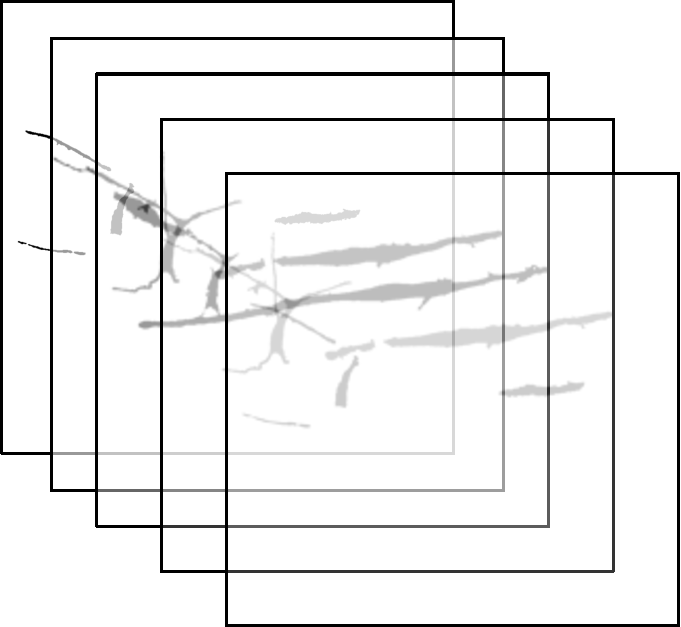
\includegraphics[height=3.5cm]{figure/ImageStack.pdf} & 
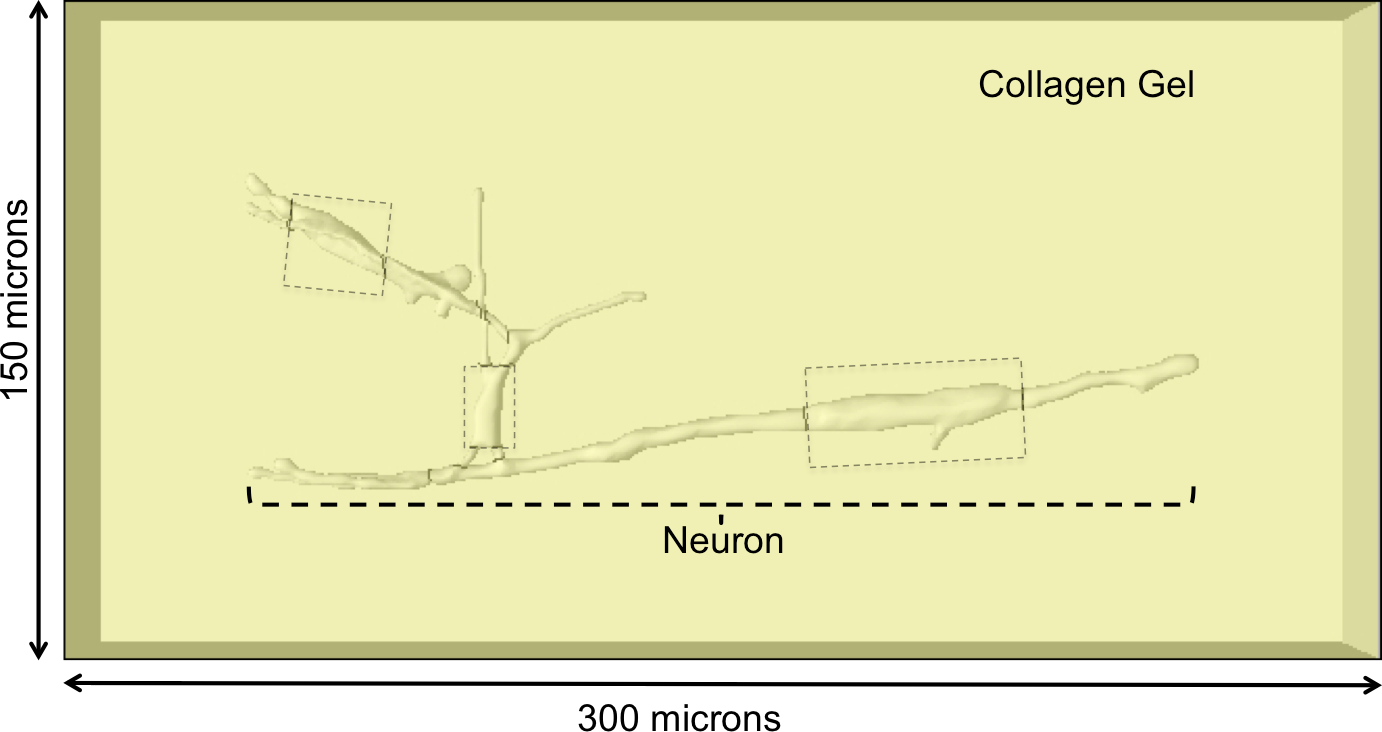
\includegraphics[height=3.5cm]{figure/neuron-in-gel_labels.pdf} &
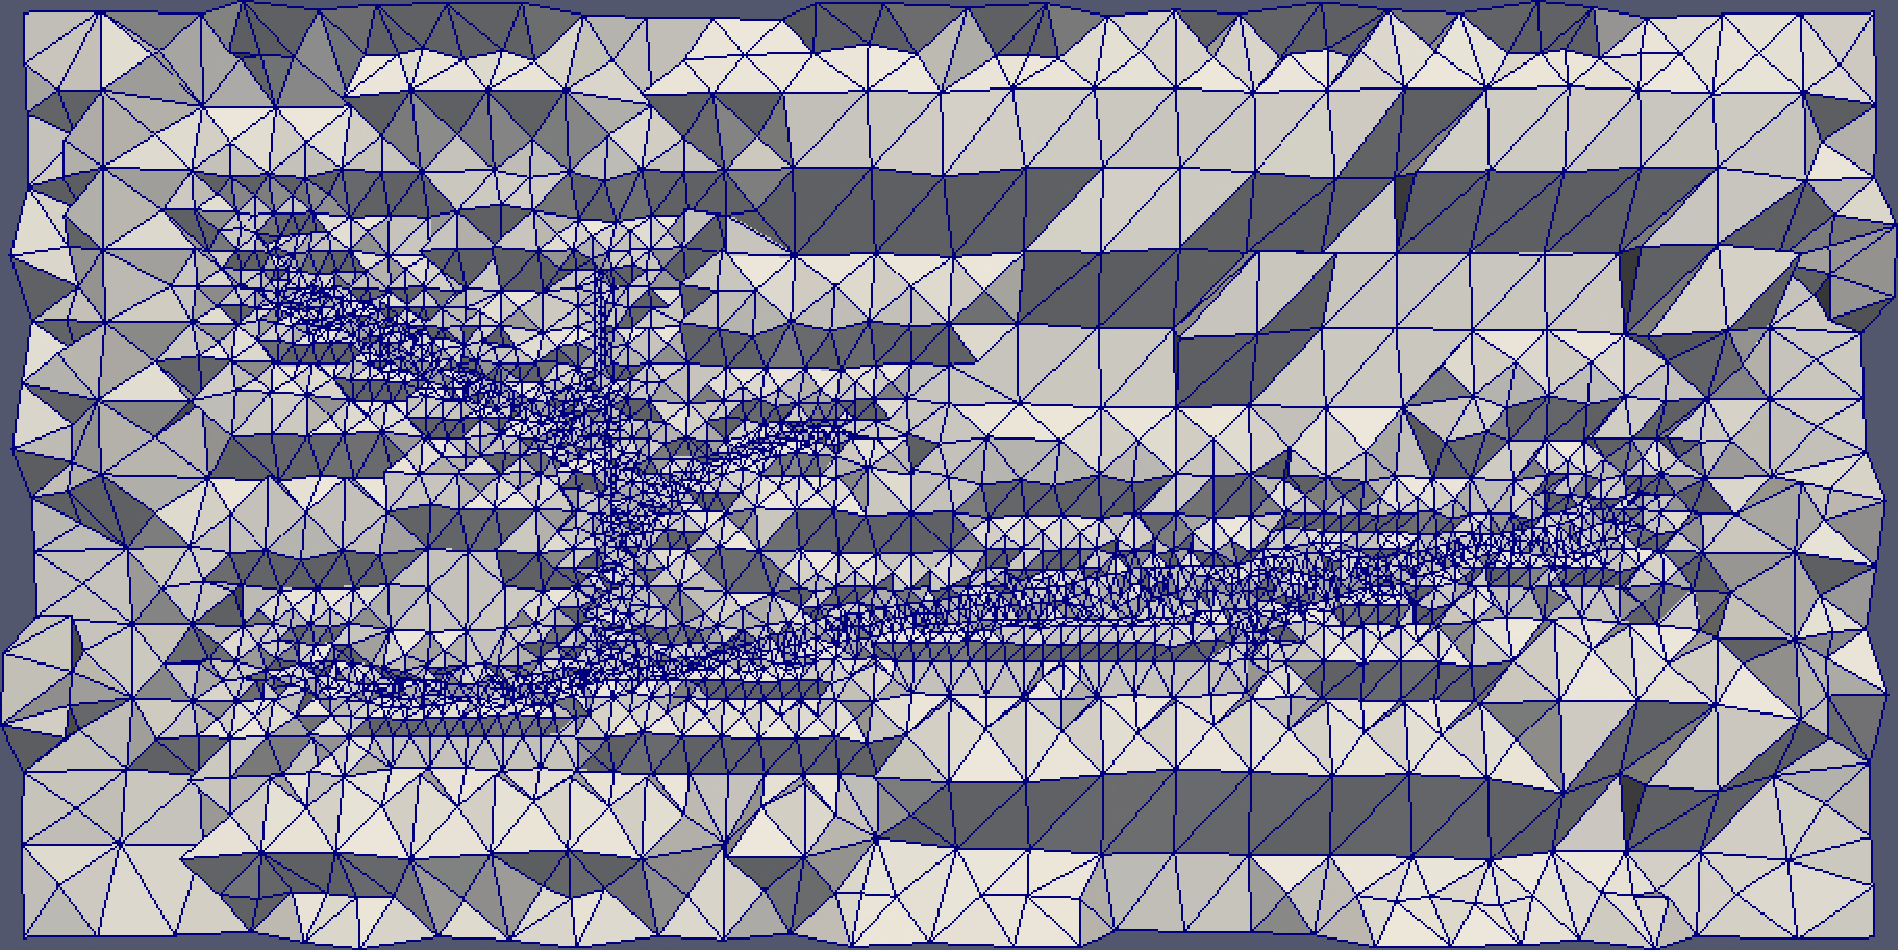
\includegraphics[height=3.5cm]{figure/neuron-in-gel_mesh.pdf} \\
(a) & (b) & (c)
\end{array}
$
\end{center}
\caption{\label{fig:image_to_model} (a) Stack of confocal images of a neuron from neuronal culture. (b) Model of neuron embedded in collagen gel that is generated from Simmetrix's \textit{ImageToModel} tool \cite{simmetrix}. Regions in the neuron that are marked with dashed rectangles are the cell bodies, while those that are not marked constitute the axons of the neuron. The region enclosing the neuron is the collagen gel. (c) Cut in neuron-in-gel model showing the mesh generated from Simmetrix meshing tools \cite{simmetrix,Shephard:2000vc}. A mesh of ~80k tetrahedral elements is used for simulations in this work.}
\end{figure}
%

%=========================================================================================================
\subsection{Multi-Scale Modeling of Collagen Gel}
Soft biological tissue consisting of collagen I has been adequately modeled using a multi-scale formulation based on volume-averaging \cite{Chandran:2007hy,Stylianopoulos:2007dp,Barocas:2007gk,Lai:2012ji,Lake:2012jm}. The multi-scale formulation consists of two scales: the microscopic scale that represents the fiber level and the macroscopic scale that represents the tissue level. The mathematical formulation for the volume-averaged multi-scale method is summarized here. For a detailed formulation, see Refs.\ \citenum{Chandran:2007hy,Stylianopoulos:2007dp}. The choice of input parameters for the multi-scale model, which are based on experimental values, is then described. 

%----------------------------------------------------------------------------------------------------------------------------------------------------------------------------------------
\subsubsection{Mathematical Formulation}
The microscopic scale is represented by a collagen network that defines the representative volume element (RVE). In our model, each RVE is generated from a Delaunay triangulation of randomly placed seed points - the edges of the triangulation represent the fibers of the network. Fiber networks with network density (total length of fibers/total number of fibers) of 100 ($\pm$ 1) were used in our simulations where the force on each fiber is
%
\begin{equation}
T_i^{(m)} = \frac{E_f A_f}{B} \left[ \exp(B\varepsilon_f^{(m)}) - 1\right],
\label{eq:fiber_force}
\end{equation}
%
where $E_f$ is the linear modulus of the collagen fiber, $A_f$ is the fiber cross-sectional area, $B$ is a constant, and $\varepsilon_f \equiv 0.5(\lambda_f - 1)$ is the fiber's Green strain, where $\lambda_f$ is the fiber stretch ratio.  The superscripts $(m)$ indicate values of the microscopic scale. The boundary deformations for each RVE is determined by the macroscopic deformation state of the macroscopic scale (down-scaling).

Upon solving for fiber-force equilibrium at each RVE, the microscopic scale is coupled to the macroscopic scale via volume averaging, where the elements of the macroscopic Cauchy stress tensor can be calculated from the equilibrium microscopic fiber forces by (up-scaling)\cite{Chandran:2007hy,Stylianopoulos:2007dp}
%
\begin{equation}
\sigma_{ij}^{(M)} = \frac{1}{V^{(m)}} \sum_{n \in bcl} {}^n x_i^{(m)} {}^n T_j^{(m)}.
\label{eq:macro_stress_discrete}
\end{equation}
%
In Eq.\ \eqref{eq:macro_stress_divergence}, ${}^nx_i^{(m)}$ is the $i^{th}$ coordinate of the $n^{th}$ cross-link on the boundary of the RVE ($bcl$) and ${}^nT_j^{(m)}$ is the $j^{th}$ component of the internal force of the $n^{th}$ cross-link on the boundary. The superscripts $(M)$ indicate values of the macroscopic scale. The Cauchy stress tensor obtained from the microscopic scale are used to solve the macroscopic force balance \cite{Chandran:2007hy,Stylianopoulos:2007dp}
%
\begin{equation}
\sigma_{ij,i}^{(M)} = \frac{1}{V^{(m)}} \int_{\partial V^{(m)}} \left( s_{ij}^{(m)} - \sigma_{ij}^{(M)} \right)u_{k,i}^{(m)} n_k dA^{(m)},
\label{eq:macro_stress_divergence}
\end{equation}
%
where $u_k^{(m)}$ is the displacement of the RVE boundary on the microscale, $n_k$ is the unit normal vector, and $s_{ij}^{(m)}$ are elements of the microscopic stress tensor. \textcolor{red}{The right-hand side of Eq.\ \eqref{eq:macro_stress_divergence} accounts for the correlation between the inhomogeneous displacement of the RVE boundary and local inhomogeneities in the stress field, which goes to zero when the RVE is fixed.}

%----------------------------------------------------------------------------------------------------------------------------------------------------------------------------------------
\subsubsection{Parameterization of fiber network}
The RVEs used in the multi-scale simulations are generated in a unit-cube compute domain that ranges from -0.5 to 0.5. In order to couple the Cauchy stress from microscopic to the macroscopic scale, the compute RVE must be properly scaled to the physical domain. In this study, the scaling between the compute and physical domains is determined by comparing the average fiber length in the RVEs to that in reconstituted collagen type I networks \cite{Lindstrom:2013gd} with collagen concentration of 2g/L. The average fiber length in the RVEs is 0.26 while that in the reconstituted collagen type I network is 1.81 $\mu$m \cite{Lindstrom:2013gd}. Based on these average lengths, a unit length in the compute  domain (average length is 0.26) is equivalent to 7 $\mu$m in the physical domain (average length is 1.81 $\mu$m); the scaling of $L=7 \ \mu$m is determined from the ratio 1.81 $\mu m$ / 0.26. Along the same line of argument, the Cauchy stresses calculated in the compute domain are scaled by $1/L^2$ to obtain Cauchy stresses for the physical domain.

To solve the microscopic scale fiber-force problem, the parameters in Eq.\ \eqref{eq:fiber_force} must be specified. The value of $A_f$ is set according to Ref.\ \citenum{Dutov:2016gu} where the fiber radius of rat tail collagen I was measured to be 162 $\mu$m. The values for $E_f$ and $B$ are set by fitting to experimentally measured stress-strain curves of rat tail collagen I gels (see Ref.\ \citenum{Zhang:2016ga} for preparation of collagen samples). \textcolor{red}{[Sijia: can you provide experimental details for measuring stress-strain curve?]}. The stress-strain curves calculated from simulation and measured experimentally are shown in Fig.\ \ref{fig:fiber_param}(a), where $E_f = 200$ kPa and $B=20$ for the RVEs used in the simulation. 
%
% (a) stress-strain curve from N2P178/1-NewParams_Cube/stress-strain folder.
% (b) fiber force curve from N2P177/LRT_Compression folder.
\begin{figure}[ht]
\begin{center}
$
\begin{array}{cc}
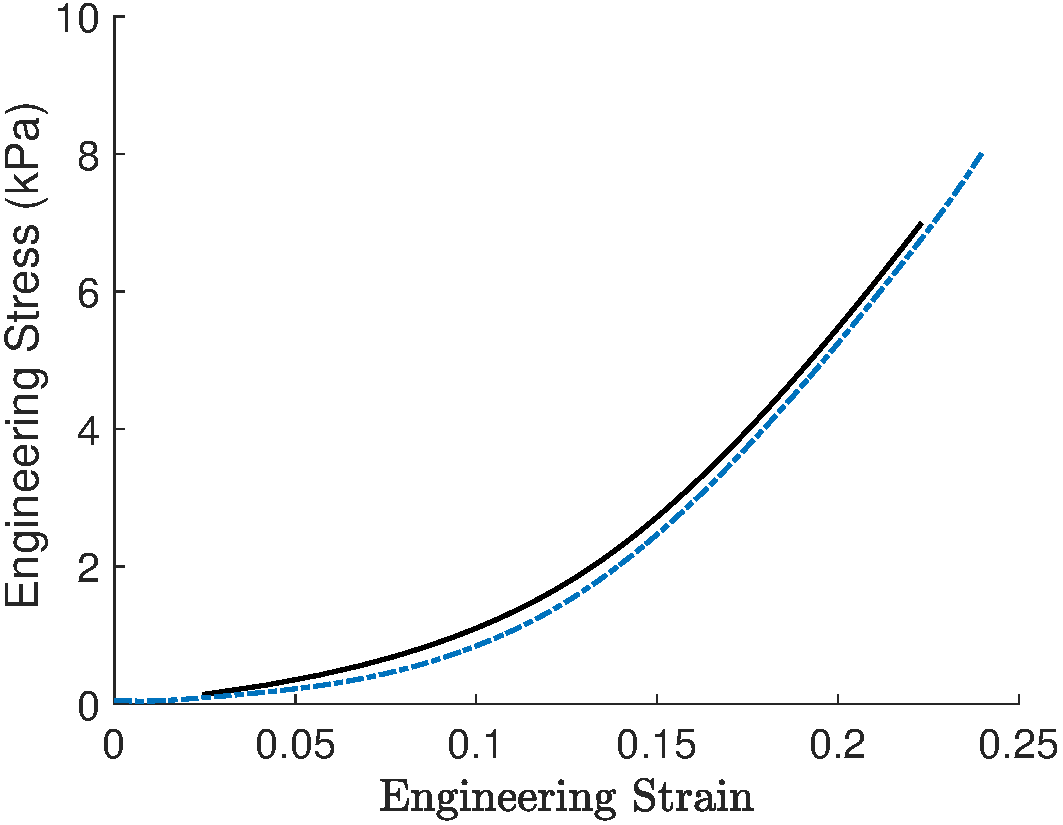
\includegraphics[height=5cm]{figure/stress_strain.pdf} &
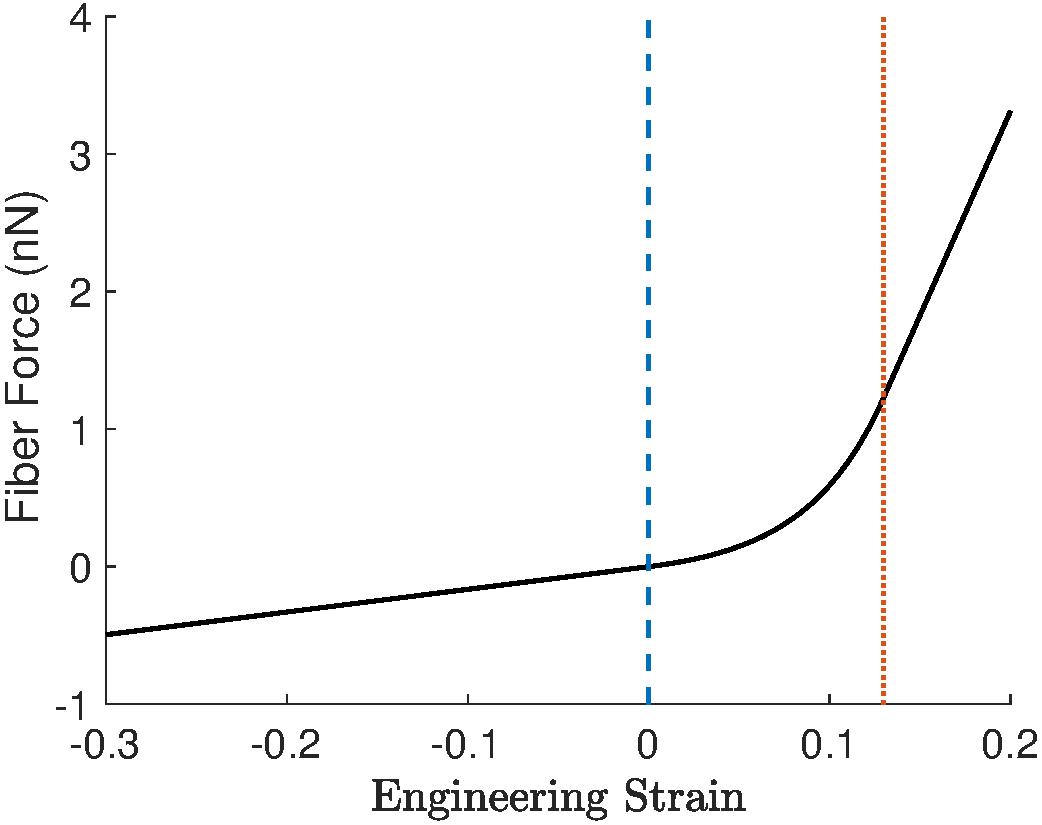
\includegraphics[height=5cm]{figure/FiberForceRelation.pdf} \\ 
(a) & (b) 
\end{array}
$
\end{center}
\caption{\label{fig:fiber_param} Plots of (a) stress-strain curve calculated from simulation (blue ``x'') and measured experimentally (black line),  and (b) fiber-force relationship for RVEs used in the simulation (blue ``x") and from Eq.\ \eqref{eq:fiber_force} (black line). The parameters of the fiber-force relationship (Eq.\ \eqref{eq:fiber_force}) are $E_f = 200$ kPa and $B=20$. The fiber force used in the simulation transitions to a linear fiber force at 13$\%$ fiber stretch - the stiffness in tension beyond 13$\%$ fiber stretch ($E_T$) is 29.7 kPa. The stiffness in compression ($E_C$) is set to the slope of Eq.\ \eqref{eq:fiber_force} at zero fiber stretch, which is 1.65 kPa.}
\end{figure}
%

In order to achieve the stress-strain fit shown in Fig.\ \ref{fig:fiber_param}(a), the exponential fiber force of Eq.\ \eqref{eq:fiber_force} is made to transition to a linear fiber-force relationship at a fiber stretch ratio of $13\%$ in tension;  the tensile stiffness for each fiber in the RVE stays constant at 29.7 kPa for fiber stretch ratios above $13\%$. Additionally, the fiber stiffness in compression is set the slope of Eq.\ \eqref{eq:fiber_force} at zero fiber stretch, which is 1.65 kPa in order to prevent the RVE fiber network from collapsing at large deformations; the fiber force from Eq.\ \eqref{eq:fiber_force} and that used in the simulations are shown in Fig.\ \ref{fig:fiber_param}(b).

The Poisson ratio is measured from the volume change of the domain via
%
\begin{equation}
\nu = \frac{1}{2}\left(1- \frac{\Delta V}{V_0}\frac{l_0}{\Delta l}\right).
\label{eq:poisson-ratio}
\end{equation}
%
The Poisson ratio as a function of applied bulk strain for the fiber-force relationship used to calculate the stress-strain curve in Fig.\ \ref{fig:fiber_param}(a) is plotted in Fig.\ \ref{fig:fiber_param2}(a). The Poisson ratio increases as a function of applied strain, and becomes larger than 0.5 at an applied strain of approximately $15\%$. The behavior of increasing Poisson ratio is consistent with experiments \cite{Vader:2009js}, however the values of Poisson ratio measured experimentally is significantly larger than what is seen in our simulations. \textcolor{red}{The difference in the Poisson ratio suggests that the simple Delaunay network used in this work is unable to fully capture all the mechanisms that arise in actual collagen gel.}
%
% (a) Poisson ratio curve from N2P178/1-NewParams_Cube/poisson-ratio folder.
% (b) Alignment curve from N2P178/1-NewParams_Cube/alignment folder.
\begin{figure}[ht]
\begin{center}
$
\begin{array}{cc}
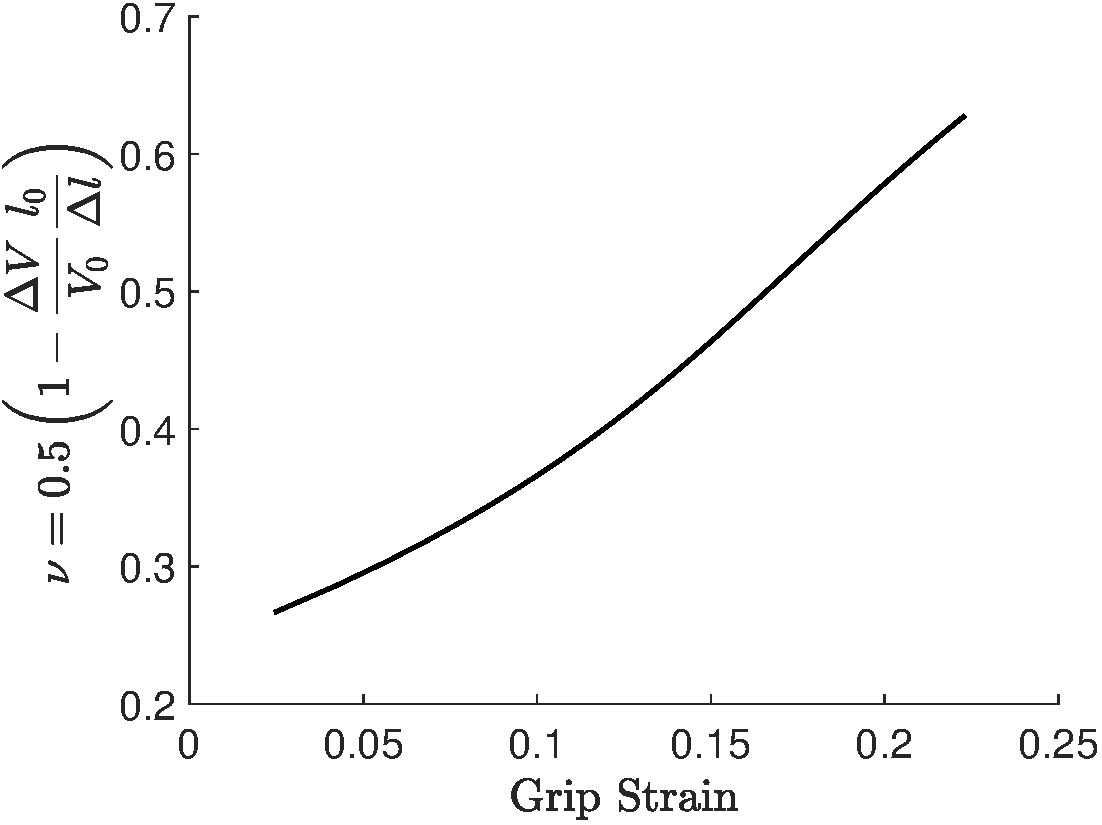
\includegraphics[height=5cm]{figure/PoissonRatio.pdf} &
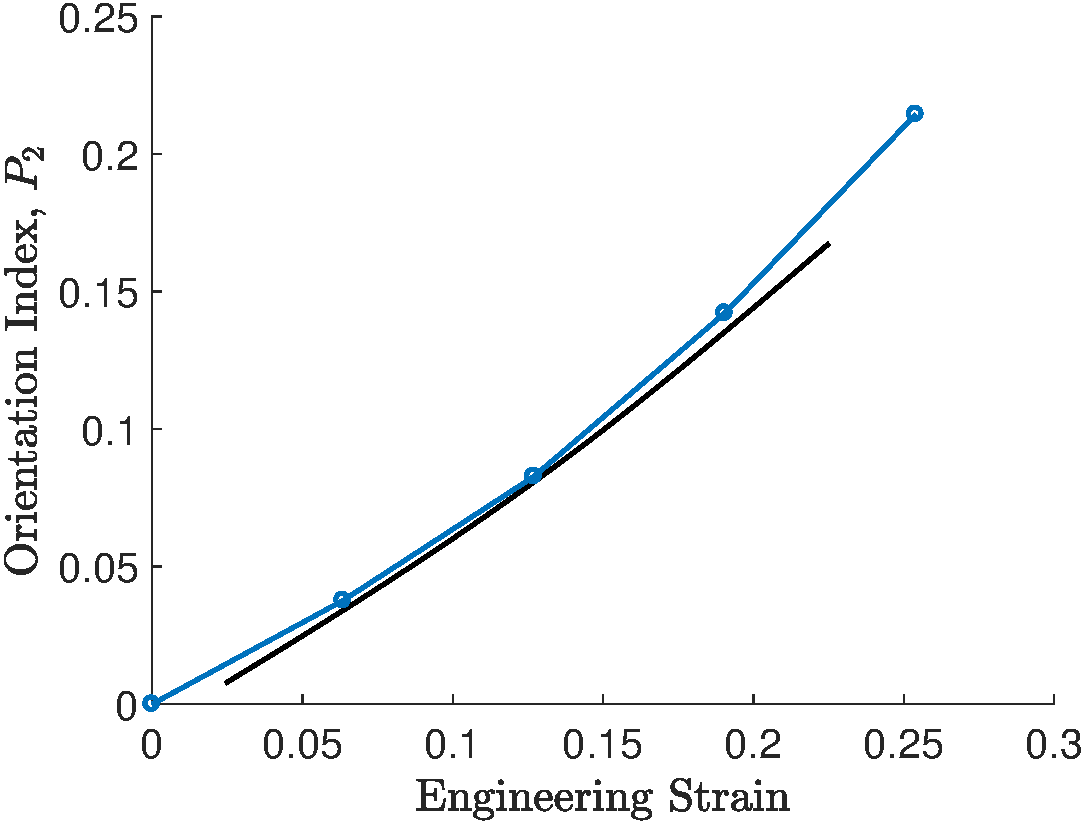
\includegraphics[height=5cm]{figure/alignment.pdf} \\ 
(a) & (b)
\end{array}
$
\end{center}
\caption{\label{fig:fiber_param2} Plots of (a) Poisson ratio calculated from simulation and (b) fiber alignment metric $P_2$ calculated from simulation (blue ``x") and measured experimentally (black line). Simulation results are calculated with fiber-force relationship used to obtain stress-strain curve in Fig.\ \ref{fig:fiber_param}.}
\end{figure}
%

The fiber alignment in innervated collagenous tissue was measured using the QPLI method \cite{Quinn:2009bf} where alignment angle $\alpha$ and retardation $\delta$ is measured in each pixel. \textcolor{red}{[Sijia: can you describe experimental setup for QPLI method?]} To compare fiber alignment that is measured experimentally and calculated from simulations, the orientation index $P_2$ is considered. The value of $P_2$ is calculated from the angle $\theta$ between fibers and the direction of alignment
%
\begin{equation}
P_2 = \frac{3 <\cos^2\theta> - 1}{2},
\label{eq:P2_simulation}
\end{equation}
%
where $<a>$ denotes the average of $a$. The value of $P_2$ ranges from 1 ($\theta=0$ or $\pi$) in which the fibers are completely aligned to -1/2 ($\theta=\pi/2$) in which the fibers are orthogonal to the alignment direction. When $P_2=0$, the fiber network is randomly oriented. The orientation index $P_2$ can be calculated from $\alpha$ and $\delta$ of the QPLI method via
%
\begin{align}
&P_2 = \int_0^{\pi} p(\theta) \cos^2\theta d\theta \nonumber\\
&p(\theta) = \frac{1}{N} \sum_{i=1}^N \left[ \frac{1-2\delta_i}{\pi} + \frac{4 \delta_i}{\pi}\cos^2(\theta - \alpha_i)\right],
\label{eq:P2_experiment}
\end{align}
%
where $\delta_i$ and $\alpha_i$ are the retardation and alignment angle, respectively, of the $i^{th}$ pixel. The fiber alignment as a function of bulk applied strain calculated from simulation and measured experimentally is plotted in Fig.\ \ref{fig:fiber_param2}(b). As expected, the fibers become more aligned as applied strain increases - the alignment in the RVE is stronger than in experiment for the same amount applied strain. \textcolor{red}{[The stronger alignment in the RVE is due to large coordination?]}

%=========================================================================================================
\subsection{Constitutive Relationship to Model Neuron}
Cross-linked microtubule bundles that are axially aligned are a major structural feature of axons, giving rise to anisotropic mechanical behavior \cite{Peter:2012fc}. To account for such mechanical anisotropy, the axons are modeled as a transversely isotropic hyperelastic material \cite{JavierBonet:2008uxa,Bonet:1998vc}. The alignment of the microtubule bundles decrease within the cell bodies causing the mechanical behavior to become more isotropic \textcolor{red}{[reference?]}. To capture such behavior, the cell bodies are modeled as a transversely isotropic hyperelastic material where the axial stiffness is a function of distance from the cell-body/axon interface - the axial stiffness is lowest at the center of the cell body. 

%----------------------------------------------------------------------------------------------------------------------------------------------------------------------------------------
\subsubsection{Mathematical Formulation}
A compressible transversely isotropic neo-Hookean model is used to model \cite{Bonet:1998vc} the axons and cell bodies of the neuron. The elements of the Cauchy stress tensor and spatial elasticity tensor can be expressed in terms of neo-Hookean (nh) and transversely isotropic (trns) components \cite{Bonet:1998vc}
%
\begin{equation}
\sigma_{ij} = \sigma^{\text{nh}}_{ij} + \sigma^{\text{trns}}_{ij} \ \ \text{ and } \ \ c_{ijkl} = c^{\text{nh}}_{ijkl} + c^{\text{trns}}_{ijkl},
\end{equation}
%
respectively, where 
%
\begin{align}
&\sigma^{\text{nh}}_{ij} = \frac{\mu}{J}(b_{ij} - \delta_{ij}) + \lambda(J-1)\delta_{ij} \nonumber\\
%
&\sigma^{\text{trns}}_{ij} = \frac{2\beta}{J}(a_r a_r - 1)\delta_{ij} + \frac{2}{J}[\alpha+2\beta\ln J+2\gamma(a_r a_r -1)]a_i a_j - \frac{\alpha}{J}(b_{is}a_s a_j+a_i b_{jr}a_r) \nonumber\\
%
&c^{\text{nh}}_{ijkl} = \lambda(2J-1)\delta_{ij}\delta_{kl} + \frac{2}{J}[\mu - \lambda J(2J-1)]\delta_{ik}\delta_{jl} \nonumber\\
%
&c^{\text{trns}}_{ijkl} = \frac{8\gamma}{J}a_i a_j a_k a_l + \frac{4\beta}{J}(a_i a_j \delta_{kl} + \delta_{ij}a_k a_l) - \frac{\alpha}{J}(a_i a_l b_{jk} + b_{ik}a_j a_l) - \frac{4\beta}{J}(a_r a_r - 1)\delta_{ik}\delta_{jl}.
\label{eq:trns_iso}
\end{align}
%
The constants of Eq.\ \eqref{eq:trns_iso} are defined as
%
\begin{align}
&\lambda = \frac{2\mu (\nu+n\nu^2)}{m} \ \ \ \ \ \gamma = \frac{E_A(1-\nu)}{8m} - \frac{\lambda+2\mu}{8} + \frac{\alpha}{2} - \beta \nonumber\\
%
&\alpha = \mu - G_A \ \ \ \ \ \ \ \ \ \ \ \ \ \ m = 1 - \nu - 2 n\nu^2 \nonumber\\
%
&\beta = \frac{\mu \nu^2(1-n)}{2m} \ \ \ \ \ \ \ \ n = \frac{E_A}{2\mu(1+\nu)},
\label{eq:trns_iso_constants}
\end{align}
%
where $\mu$ is the shear modulus, $G_A$ is the axial shear modulus, $\nu$ is the Poisson ratio, and $E_A$ is axial Young's modulus. In the cell bodies, the axial Young's modulus decreases as one moves away from the cell-body/axon interface towards the interior of the cell body by 
%
\begin{equation}
E_A^{cell} = \left(1 - \frac{D}{a}\right)E_A,
\label{eq:cellEA}
\end{equation}
%
where $D$ is the distance of an interior point of the cell body to the closest cell-body/axon interface and $a$ is a constant that dictates how quickly $E_A$ decreases when moving from the cell-body/axon interface towards the interior of the cell body. The axial stiffness decreases more quickly for smaller values of $a$.

%----------------------------------------------------------------------------------------------------------------------------------------------------------------------------------------
\subsubsection{Parameterization of cell body and axon}
The value of $E_A$ is based on the study by Peter and Mofrad \cite{Peter:2012fc}, where the mechanical behavior of axonal microtubule bundles under tension were simulated with a discrete bead-spring model. To apply their results for microtubule bundles to our neuron model, we assume that only the microtubule bundles carry force in the axon and that the stress of the microtubule bundles can be redistributed over the cross-sectional area of the axon. Based on these assumptions, the axial stiffness of the axon can be related to the axial stiffness of the microtubule bundles ($E_{MTb}$) by
%
\begin{equation}
E_A = \frac{E_{MTb} A_{MTb}}{A_A},
\label{eq:EA_EMTb_relation}
\end{equation}
%
where $A_{MTb}$ and $A_A$ are the cross-sectional areas of the microtubule bundle and axon, respectively. 

The cross-sectional areas and elastic moduli for the axon are listed in table \ref{table:axon_parameters}. The transverse stiffness of the cell body and axon is set to 1.5 kPa according to AFM measurements of the neuron soma from Simon et al. \cite{Simon:2016ig}. We assume that the axon and cell body have the same mechanical behavior in the transverse direction.
%%%%%%%%%%%%%%%%%%%%%%%%%%%%%%%%%%%%%%%%%%%%%%%%%%%%%%%%
\begin{table}[ht]
\begin{center}
\begin{tabular}{ l c l }
\hline \hline
$A_{MTb}$ & 0.344 $\mu$m${}^2$ & calculated according to schematic in Fig.\ \ref{fig:microtubule_bundle}. \\
$A_A$ & 19.6 $\mu$m${}^2$ & calculated from average axon diameter. \\
$E_{MTb}$ & $4\times 10^{4}$ kPa & this is an average value - the elastic modulus of the microtubule bundle increases linearly with strain \cite{Peter:2012fc}. \\
$E_A$ & 70 kPa  & calculated from Eq.\ \eqref{eq:EA_EMTb_relation}. \\ \hline \hline
\end{tabular}
\end{center}
\caption{Parameters for axon structure.}
\label{table:axon_parameters}
\end{table}
%%%%%%%%%%%%%%%%%%%%%%%%%%%%%%%%%%%%%%%%%%%%%%%%%%%%%%%%
%
%image from BiotissueMeetings/Biotissue_Meeting_3_17_17
\begin{figure}[ht]
\begin{center}
$
\begin{array}{c}
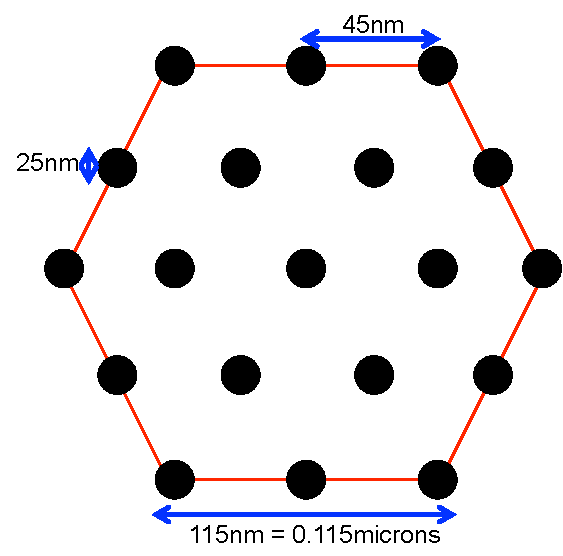
\includegraphics[height=5cm]{figure/microtubule_bundle.pdf} 
\end{array}
$
\end{center}
\caption{\label{fig:microtubule_bundle} Cross-section of microtubule bundle based on dimensions from Ref.\ \citenum{Peter:2012fc}. Diameter of a microtubule (black dot) is 25nm and edge-to-edge spacing between microtubules is 20nm. Figure is not drawn to scale. }
\end{figure}
%

%=========================================================================================================
\subsection{Multi-scale Implementation via AMSI}
\textcolor{red}{Bill can briefly describe implementation of AMSI here.}

%%%%%%%%%%%%%%%%%%%%%%%%%%%%%%%%%%%%%%%%%%%%%%%%%%%%%%%%%%%%%%%%%%%%%%
\section{Results and Discussion}
To gain insight about the interactions within innervated collagenous tissue, we examine the mechanical behavior of our embedded neuron model when the surrounding collagen gel is loaded in different directions. The load directions relative to the neuron structure are illustrated in the schematic of Fig.\ \ref{fig:analysis_schematic}(a). Loads of up to 20$\%$ bulk strain are considered to capture the behavior below and above the pain threshold of $16\%$ bulk strain \cite{Zhang:2016ga}. For the results in this section, $a=30$ is used for $E_A^{cell}$ in Eq.\ \eqref{eq:cellEA}. The resulting axial Young's modulus in the neuron is plotted in Fig.\ \ref{fig:analysis_schematic}(b).
%
%image for axial young's modulus from N2P178/3-Neuron_FT folder
\begin{figure}[ht]
\begin{center}
$
\begin{array}{cc}
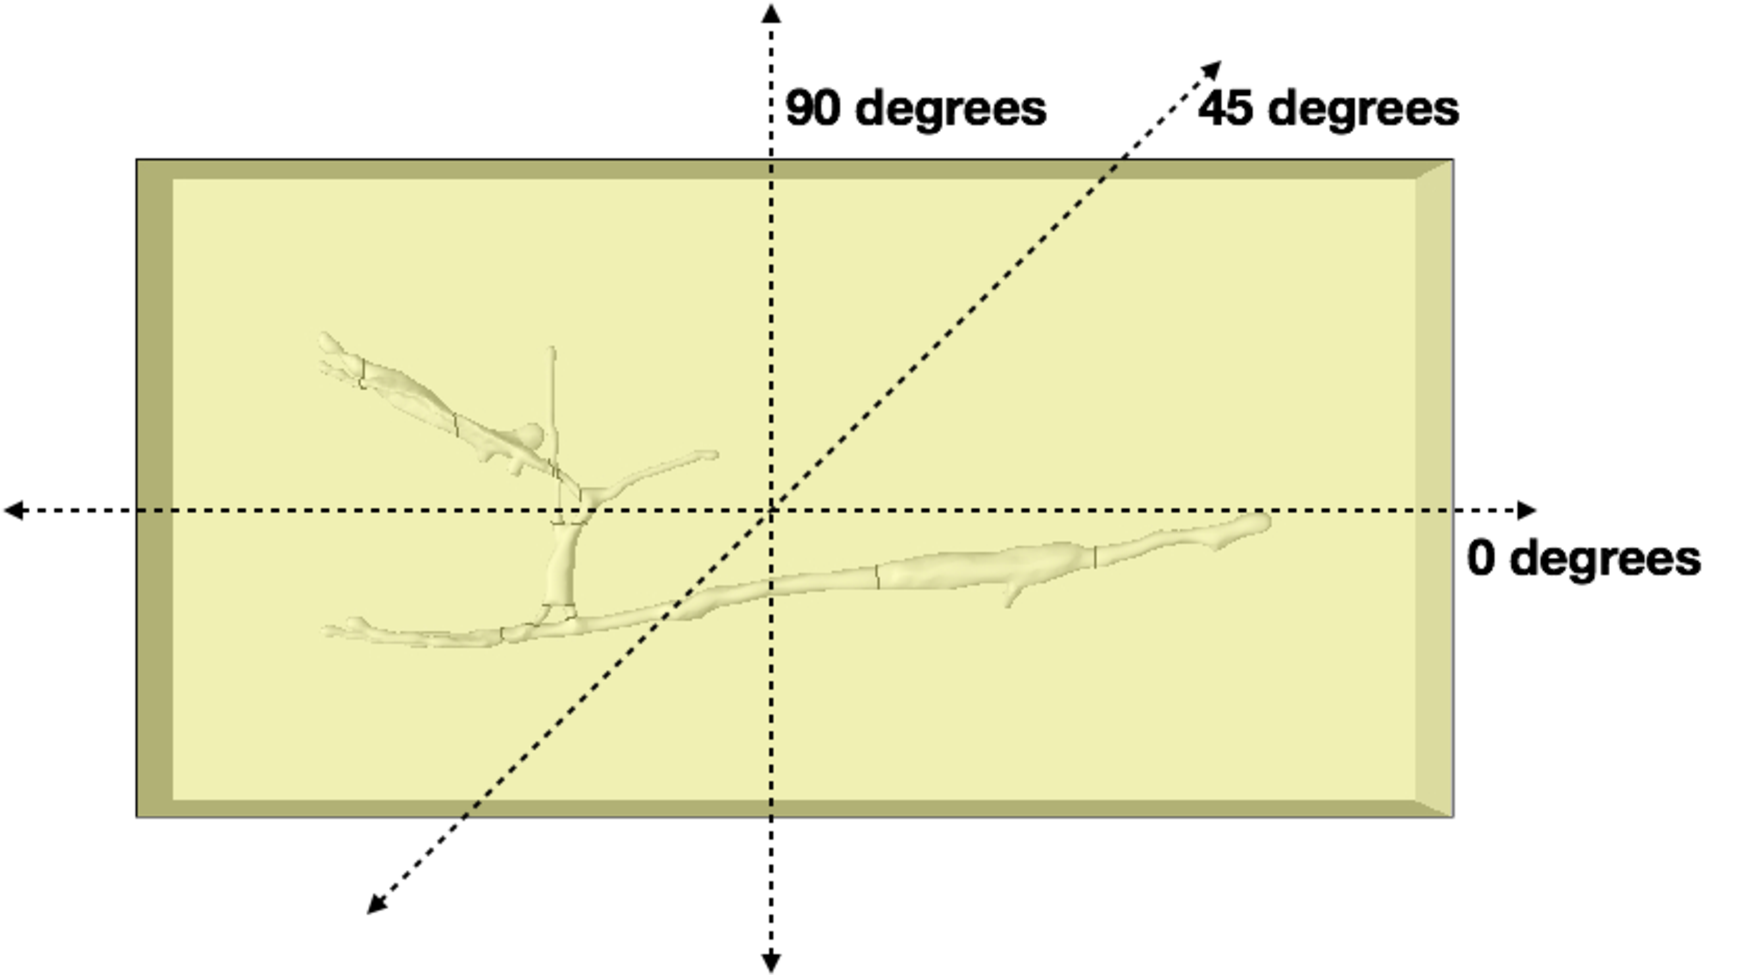
\includegraphics[height=4cm]{figure/AngleLoadingSchematic.pdf} &
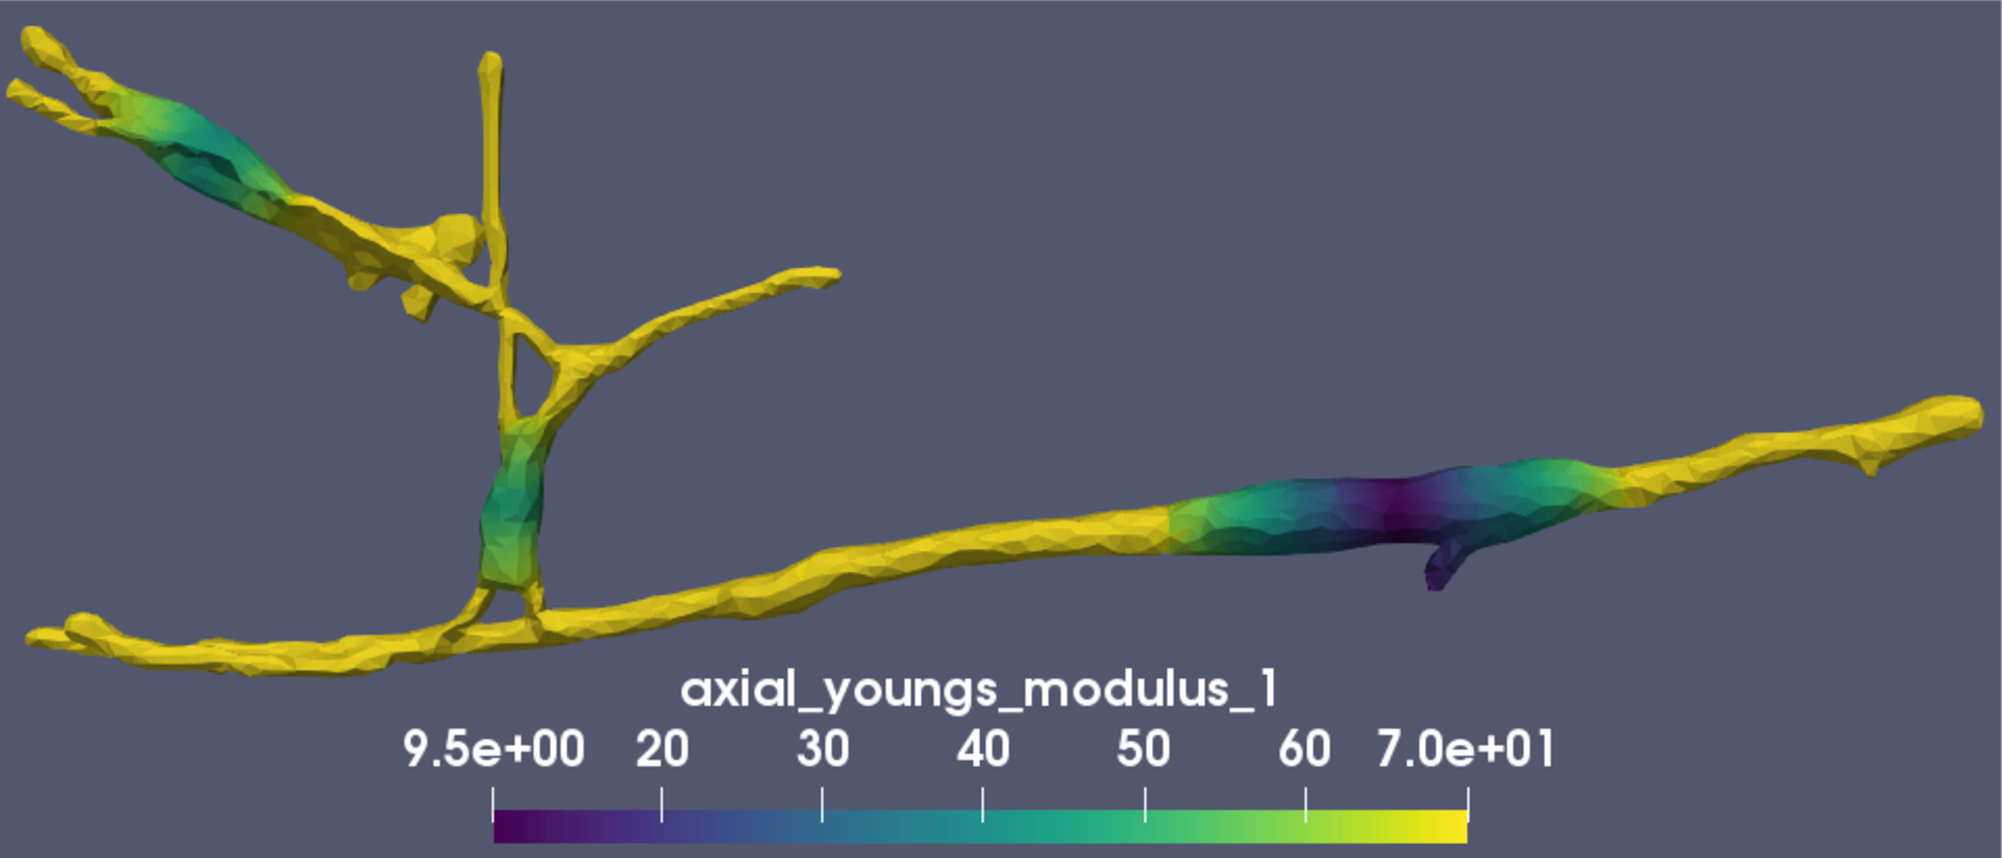
\includegraphics[height=3.5cm]{figure/axial_youngs_modulus_a30.pdf} \\
(a) & (b)
\end{array}
$
\end{center}
\caption{\label{fig:analysis_schematic} (a) Schematic showing load directions corresponding to 0 (solid black arrows), 45 (dotted arrows), and 90 (stripped arrows) degrees relative to the neuron structure. (b) Plot of axial Young's modulus for $a=40$ in Eq.\ \eqref{eq:cellEA} and $E_A=70$ kPa.}
\end{figure}
%
%=========================================================================================================
\subsection{Strain Distributions in Neuron}
The complementary cumulative distribution function (cdf) for the maximum principal strain is calculated for the neuron structure via
%
\begin{equation}
1 - cdf(x) = 1 - \sum_{i=1}^x f(i) = 1 - Pr[X \le x],
\label{eq:comp_cdf}
\end{equation}
%
where $f$ is a probability density function and $X$ is a random variable (maximum principal strain in our case). Equation \ref{eq:comp_cdf} measures the probability that the neuron experiences a maximum principal strain of \textit{at least} $x$. The complementary cdf for the neuron structure is shown in Fig.\ \ref{fig:neuron_cdf} for different angles of applied load.
%
\begin{figure}[ht]
\begin{center}
$
\begin{array}{ccc}
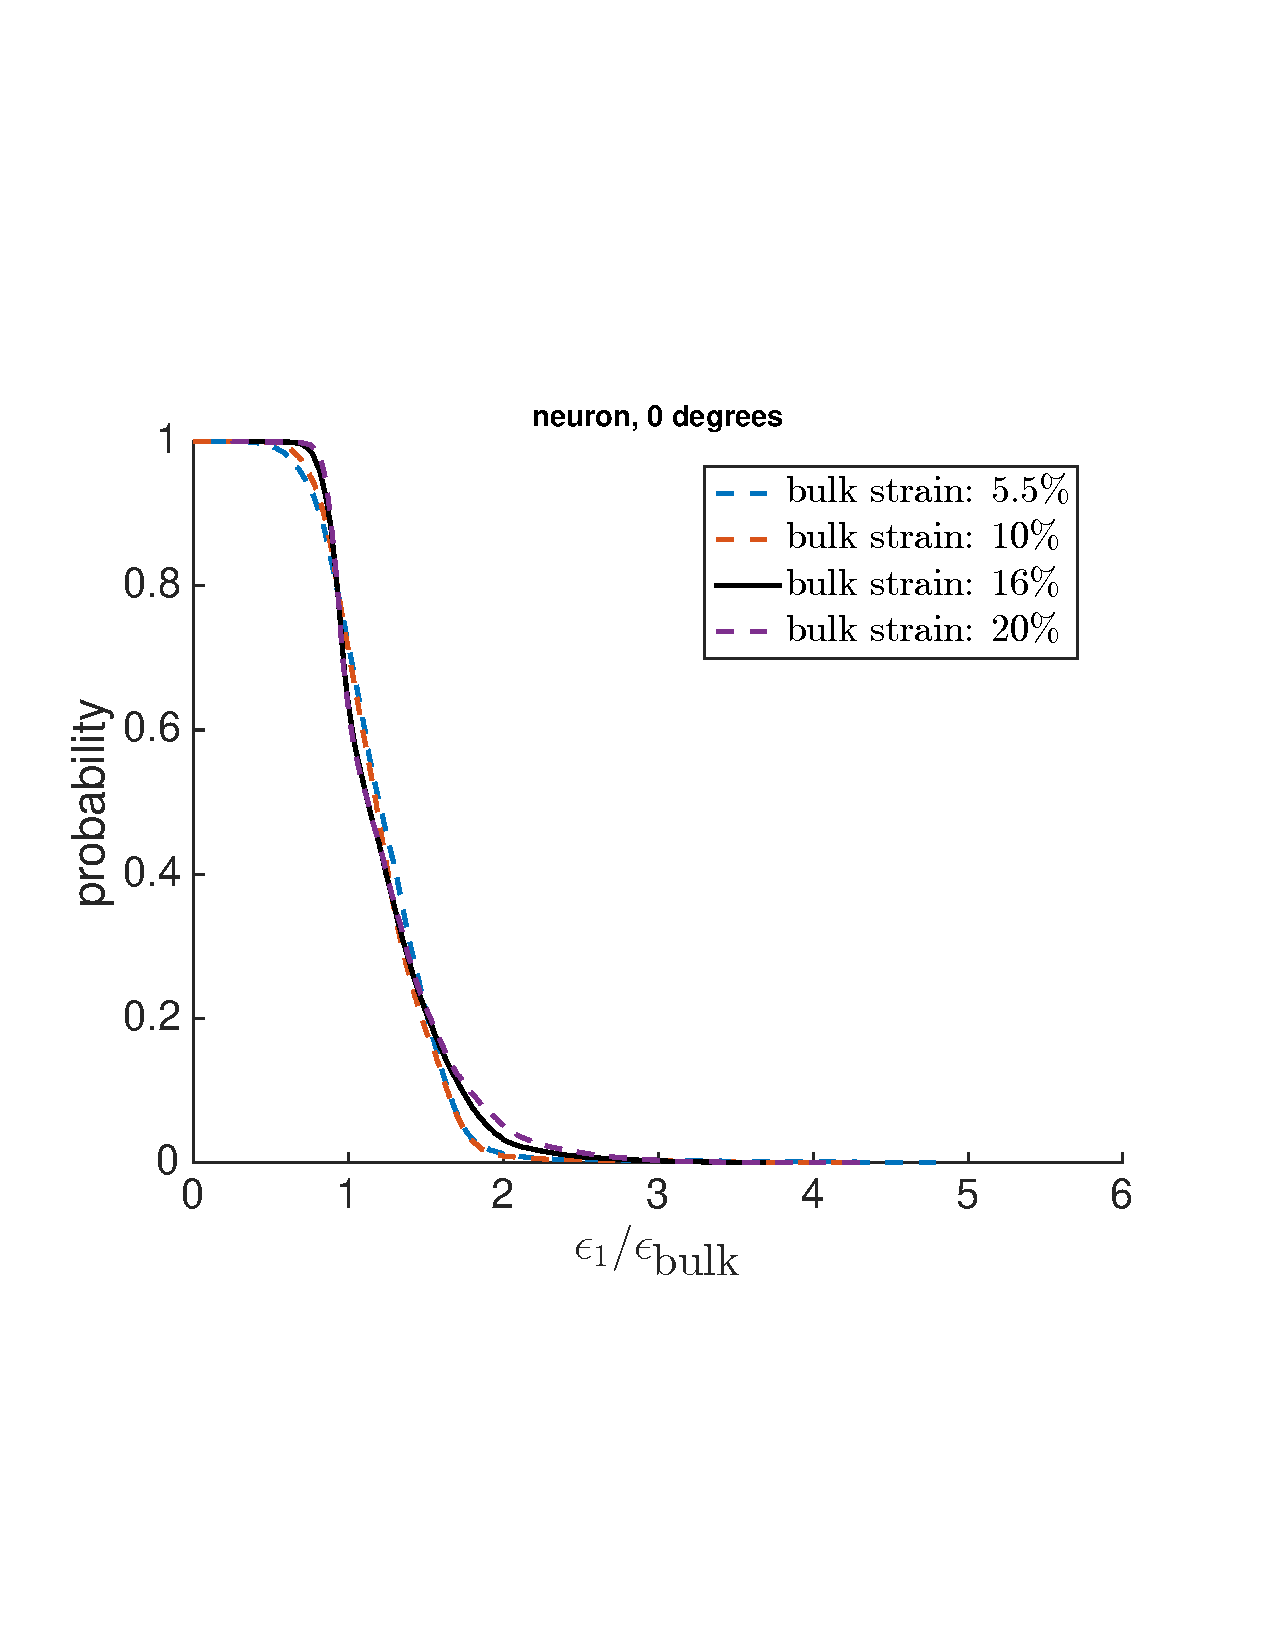
\includegraphics[height=4cm]{figure/rot0_FT50_128_1920_cdf_neuron_compare_stps.pdf} &
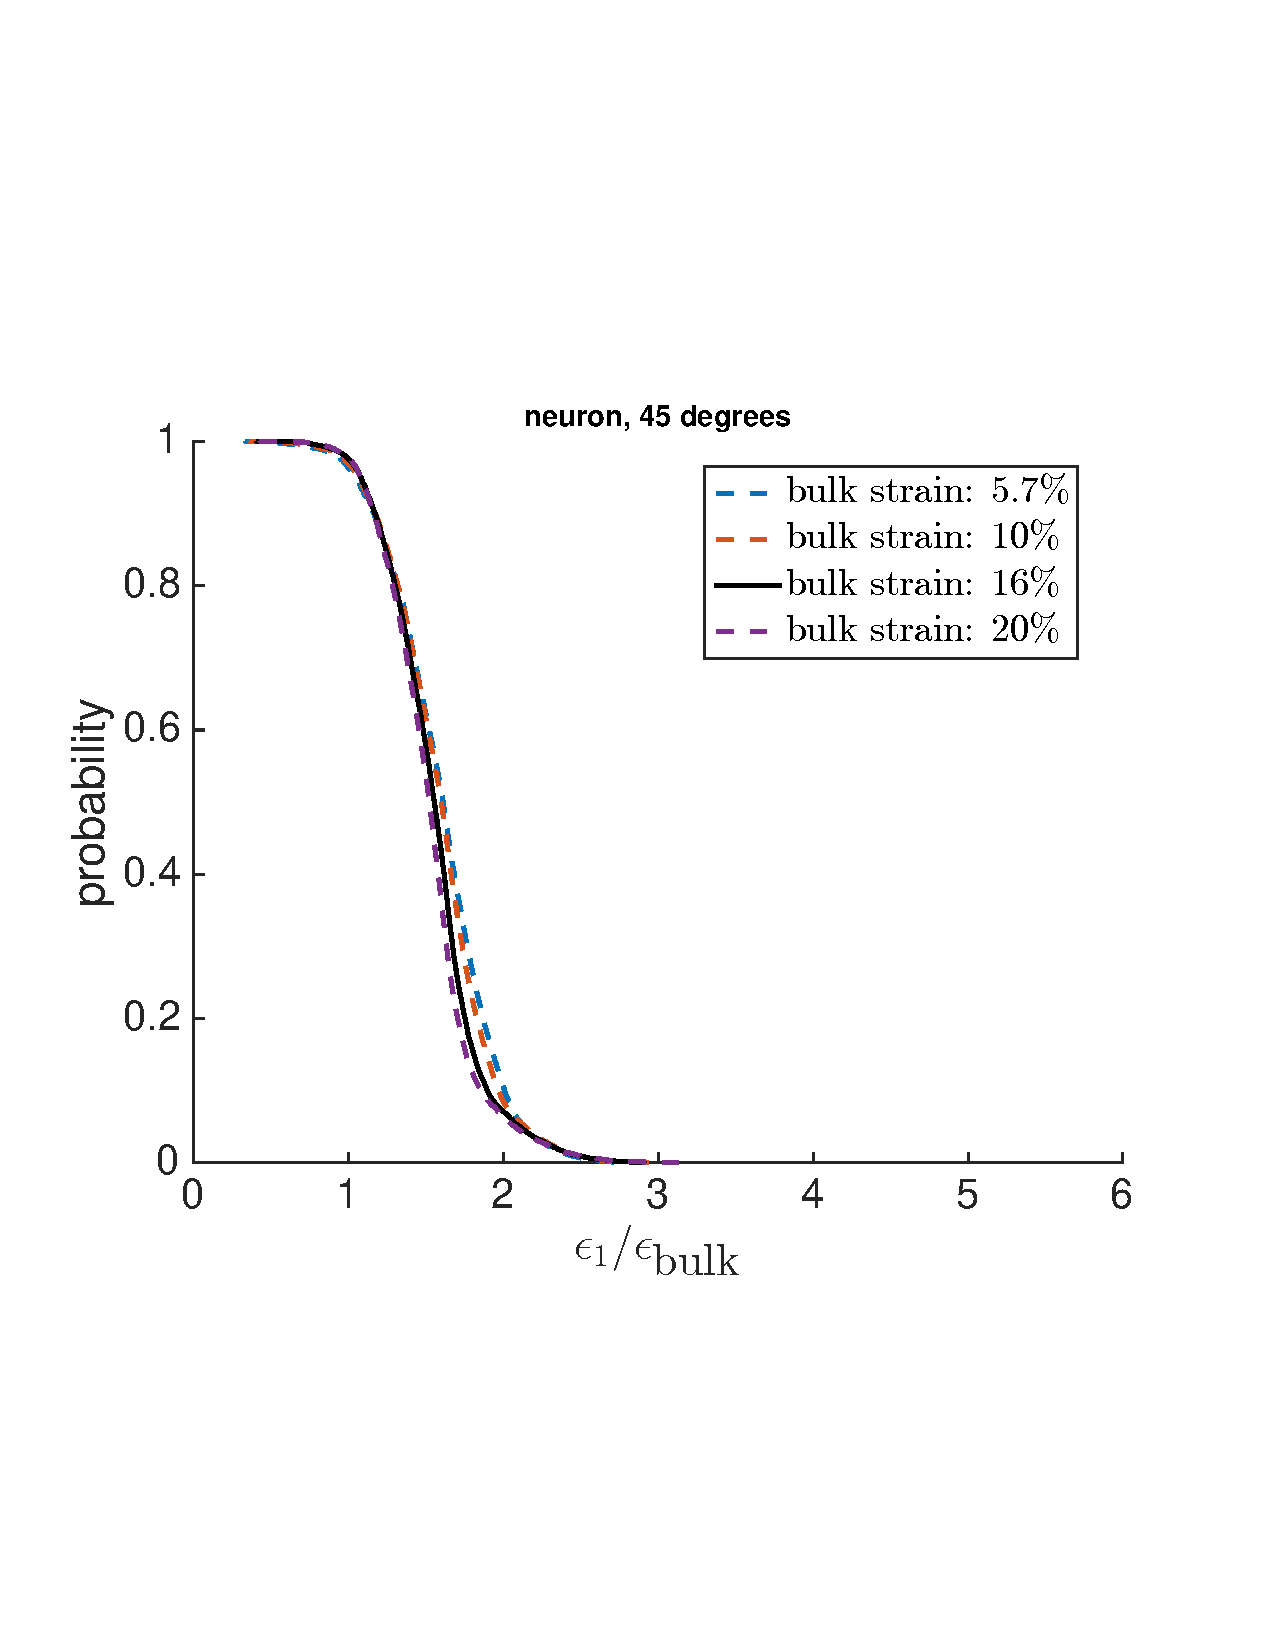
\includegraphics[height=4cm]{figure/rot45_FT50_128_1920_cdf_neuron_compare_stps.pdf} &
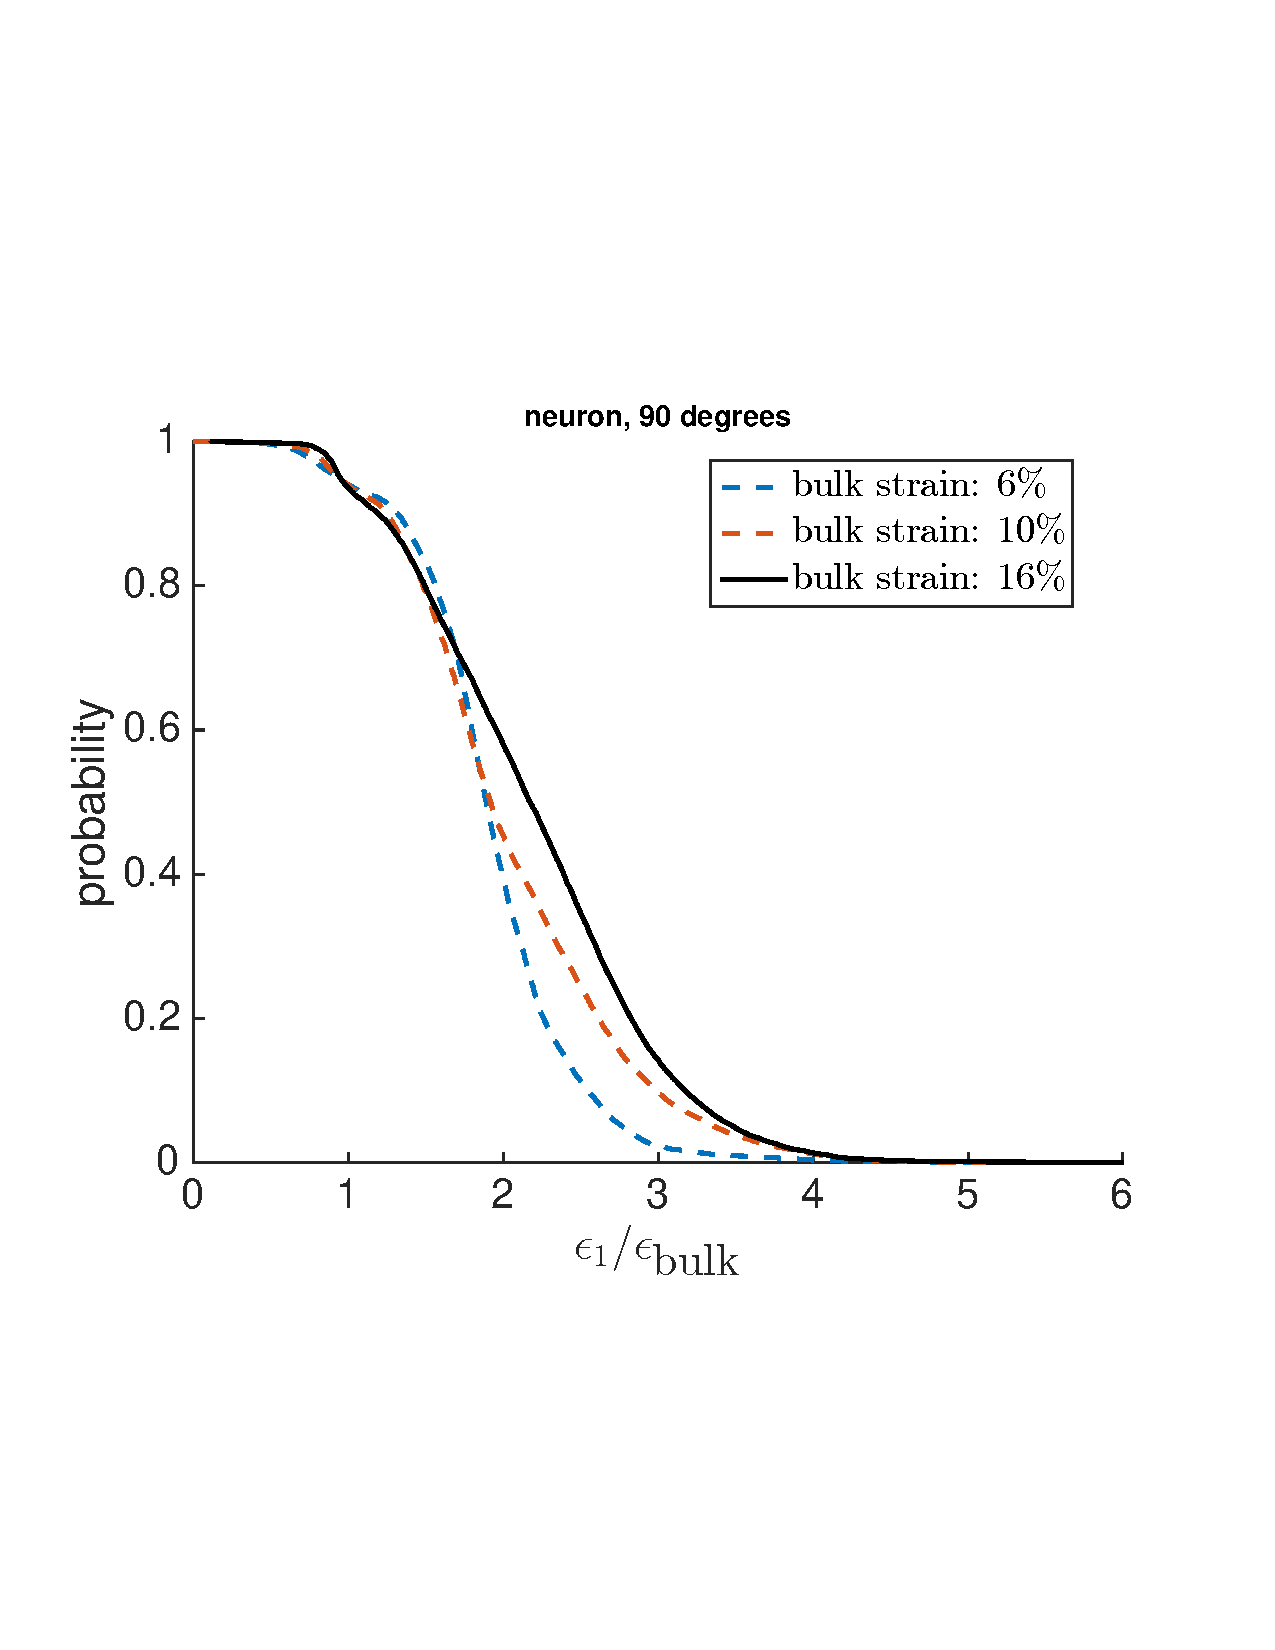
\includegraphics[height=4cm]{figure/rot90_FT_dspBC50_a30_128_1920_cdf_neuron_compare_stps_farfield.pdf} \\
(a) & (b) & (c)
\end{array}
$
\end{center}
\caption{\label{fig:neuron_cdf} Complementary cdf of normalized maximum principal strain ($\varepsilon_1$) in the neuron for applied loads at (a) 0 degrees, (b) 45 degrees, and (c) 90 degrees. For each angle, the complementary cdf for bulk strains below, above, and at the pain threshold (16$\%$) are shown. The values of $\varepsilon_1$ are normalized by the applied bulk strain ($\varepsilon_{\text{bulk}}$) that is applied to the surrounding collagen gel.  }
\end{figure}
%
For all angles of applied load considered, the neuron experiences local strains that are significantly larger than the applied load on the surrounding collagen gel (see tails of distribution in Fig.\ \ref{fig:neuron_cdf}). The neuron experiences the largest local strain of more than 6 times the bulk strain for applied loads at 90 degrees and the lowest local strain of approximately 3 times the bulk strain for an applied load at 45 degrees.

The shape and spread of the strain distribution in the neuron varies with the bulk strain for an applied load at 90 degrees - the spread of the distribution increases with larger bulk strain. In contrast, the shape and spread of the strain distribution in the neuron remains relatively constant for applied loads at 0 and 45 degrees. Interestingly, for all cases, the distributions converge to the distribution corresponding to the load at the pain threshold (16$\%$), i.e., the distribution at 20$\%$ bulk strain is essentially identical to that corresponding to the pain threshold \textcolor{red}{(need to verify for the applied load at 90 degrees case)}.  

Additional insight can be gained by separating the strain distribution of the neuron into contributions from the cell bodies and axons. The complimentary cdfs for the cell bodies and axons are plotted in Fig.\ \ref{fig:components_cdf}.
%
\begin{figure}[ht]
\begin{center}
$
\begin{array}{ccc}
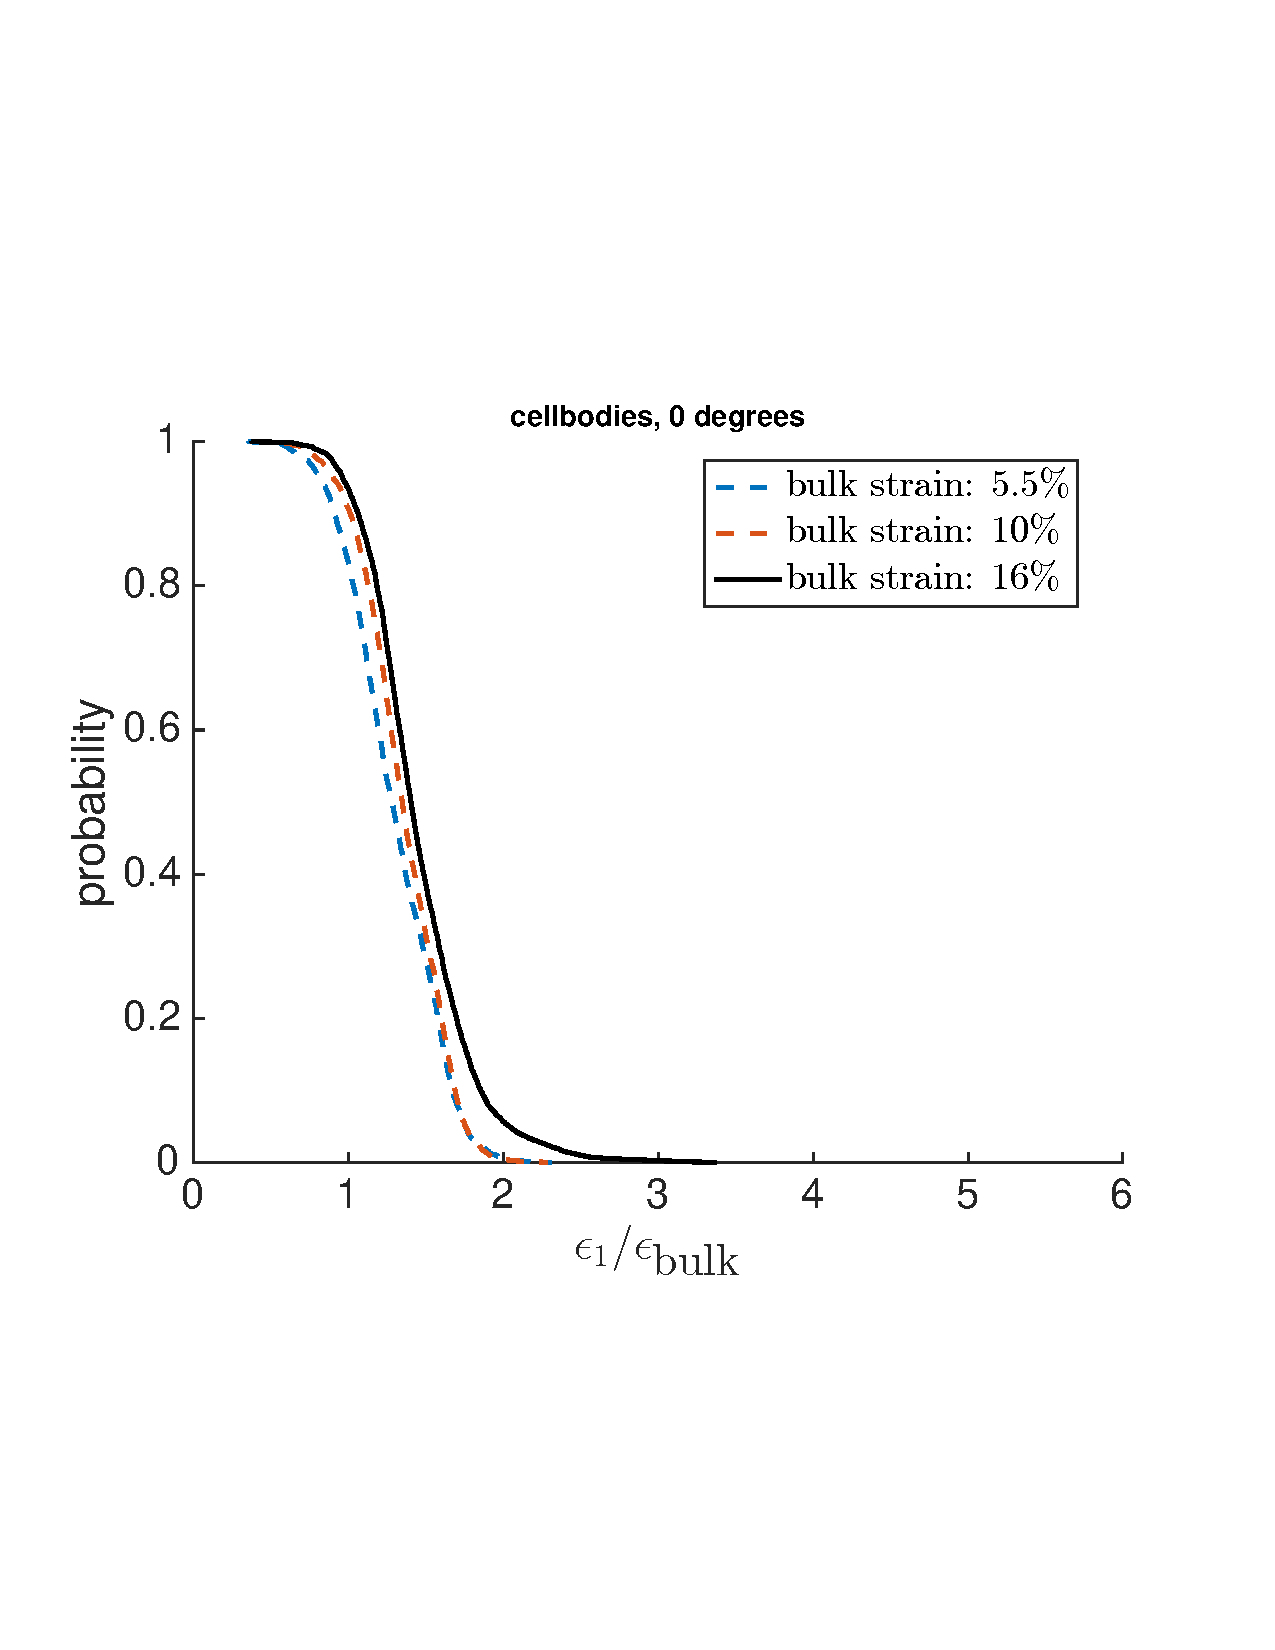
\includegraphics[height=4cm]{figure/rot0_FT50_128_1920_cdf_cellbodies_compare_stps.pdf} & 
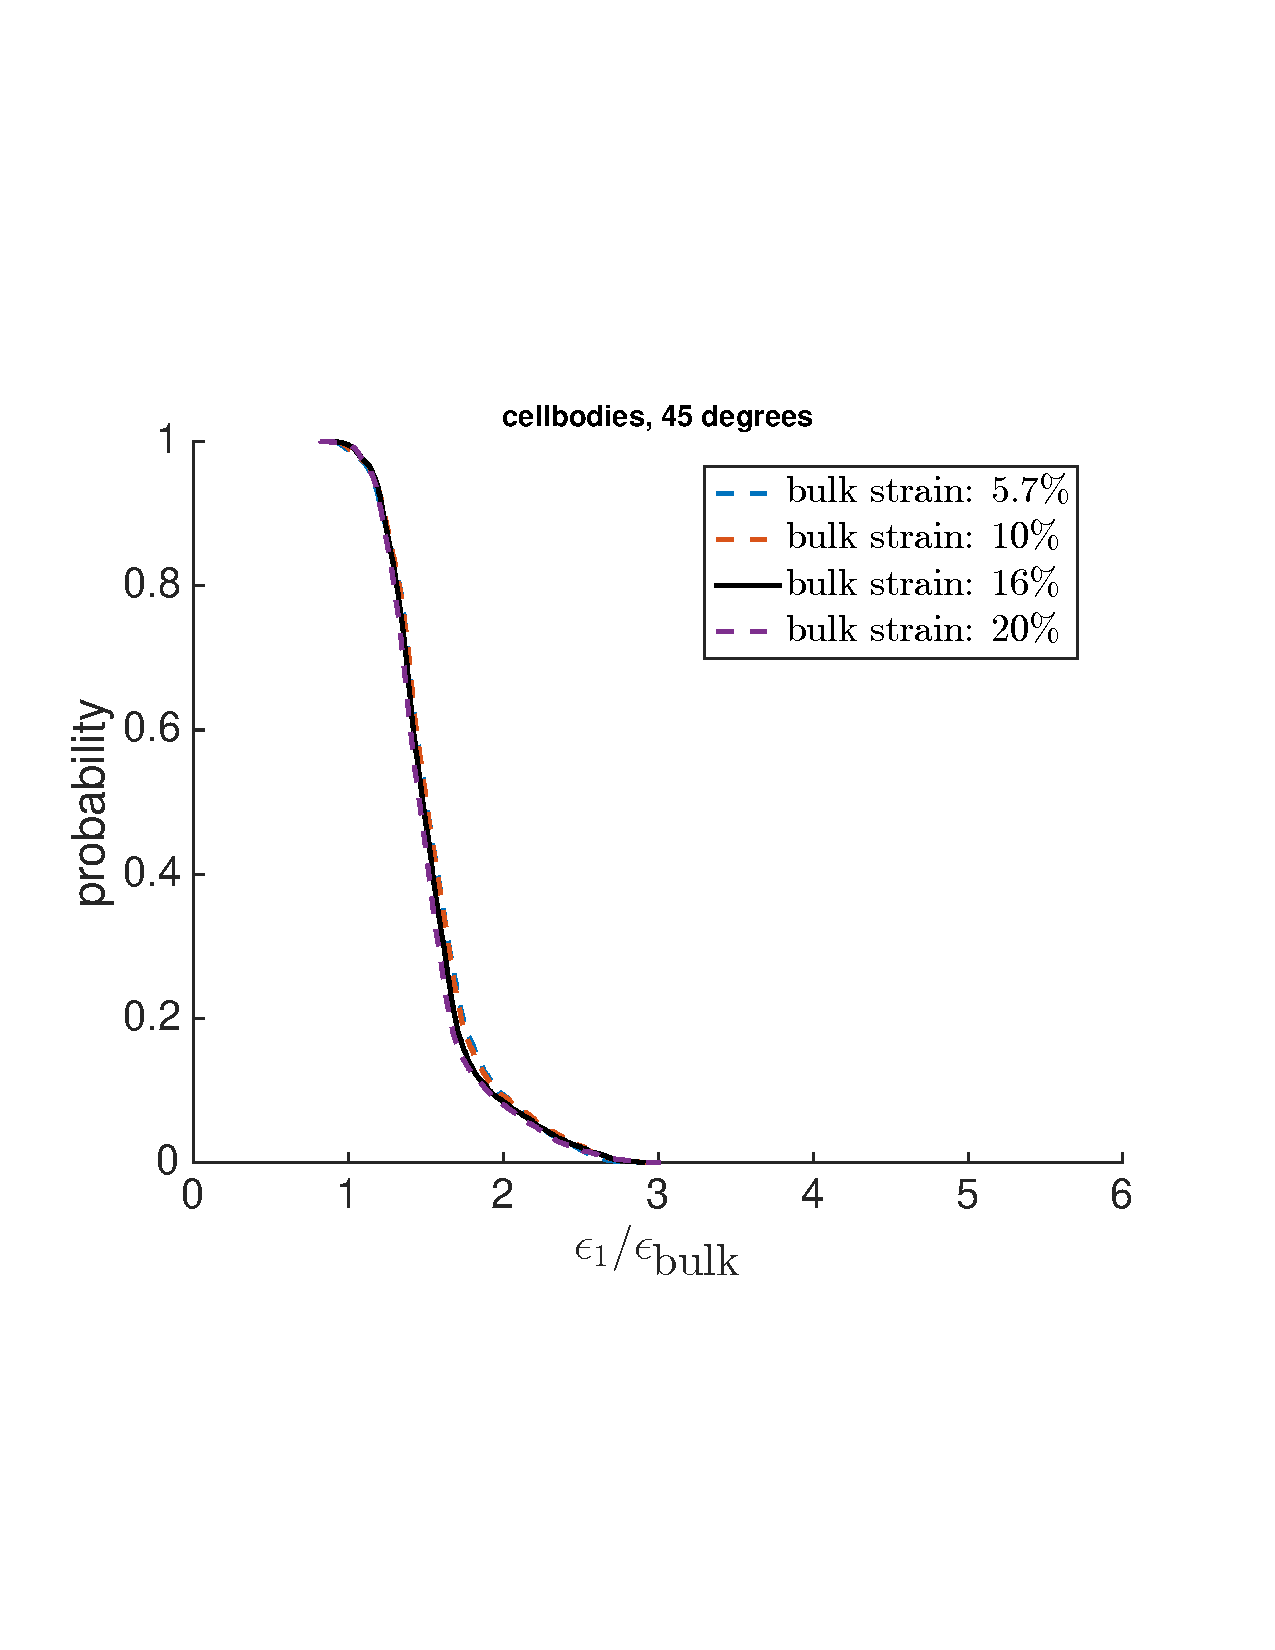
\includegraphics[height=4cm]{figure/rot45_FT50_128_1920_cdf_cellbodies_compare_stps.pdf} & 
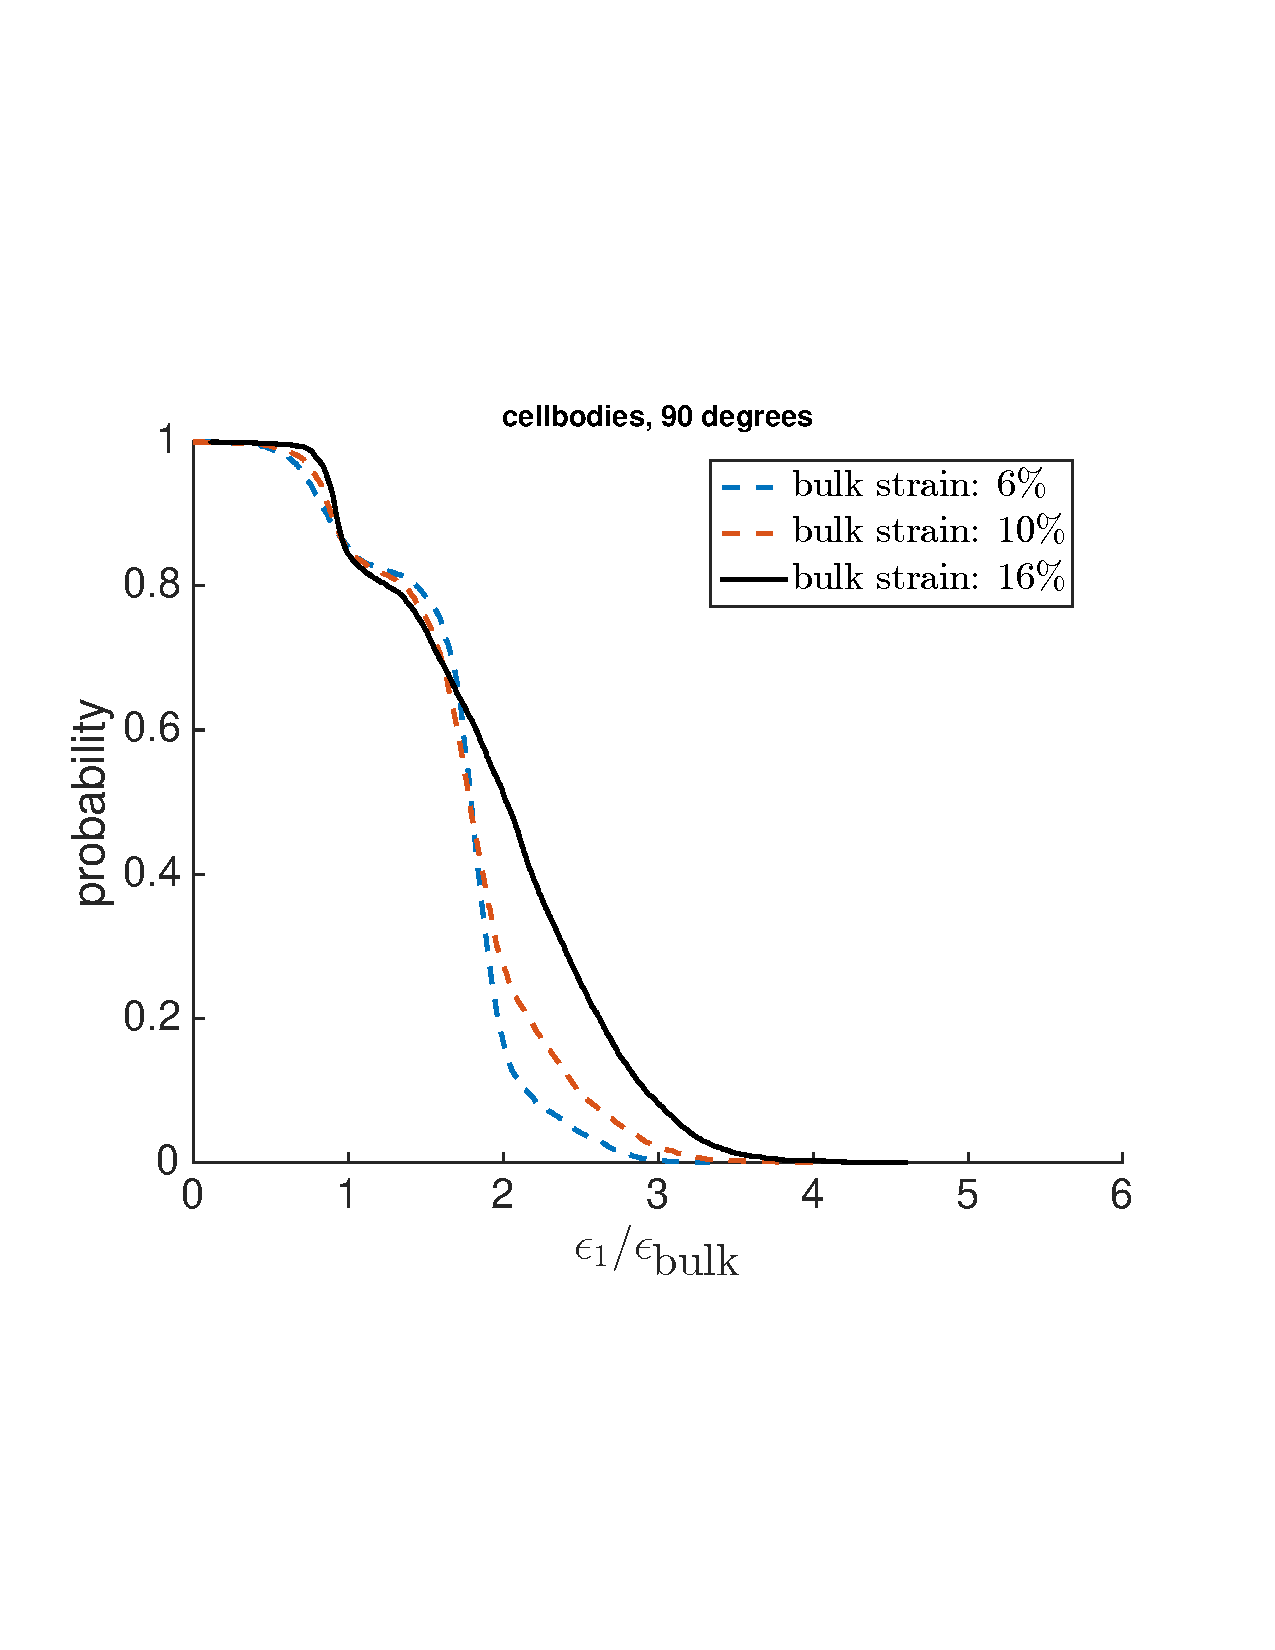
\includegraphics[height=4cm]{figure/rot90_FT_dspBC50_a30_128_1920_cdf_cellbodies_compare_stps_farfield.pdf} \\
(a) & (b) & (c) \\
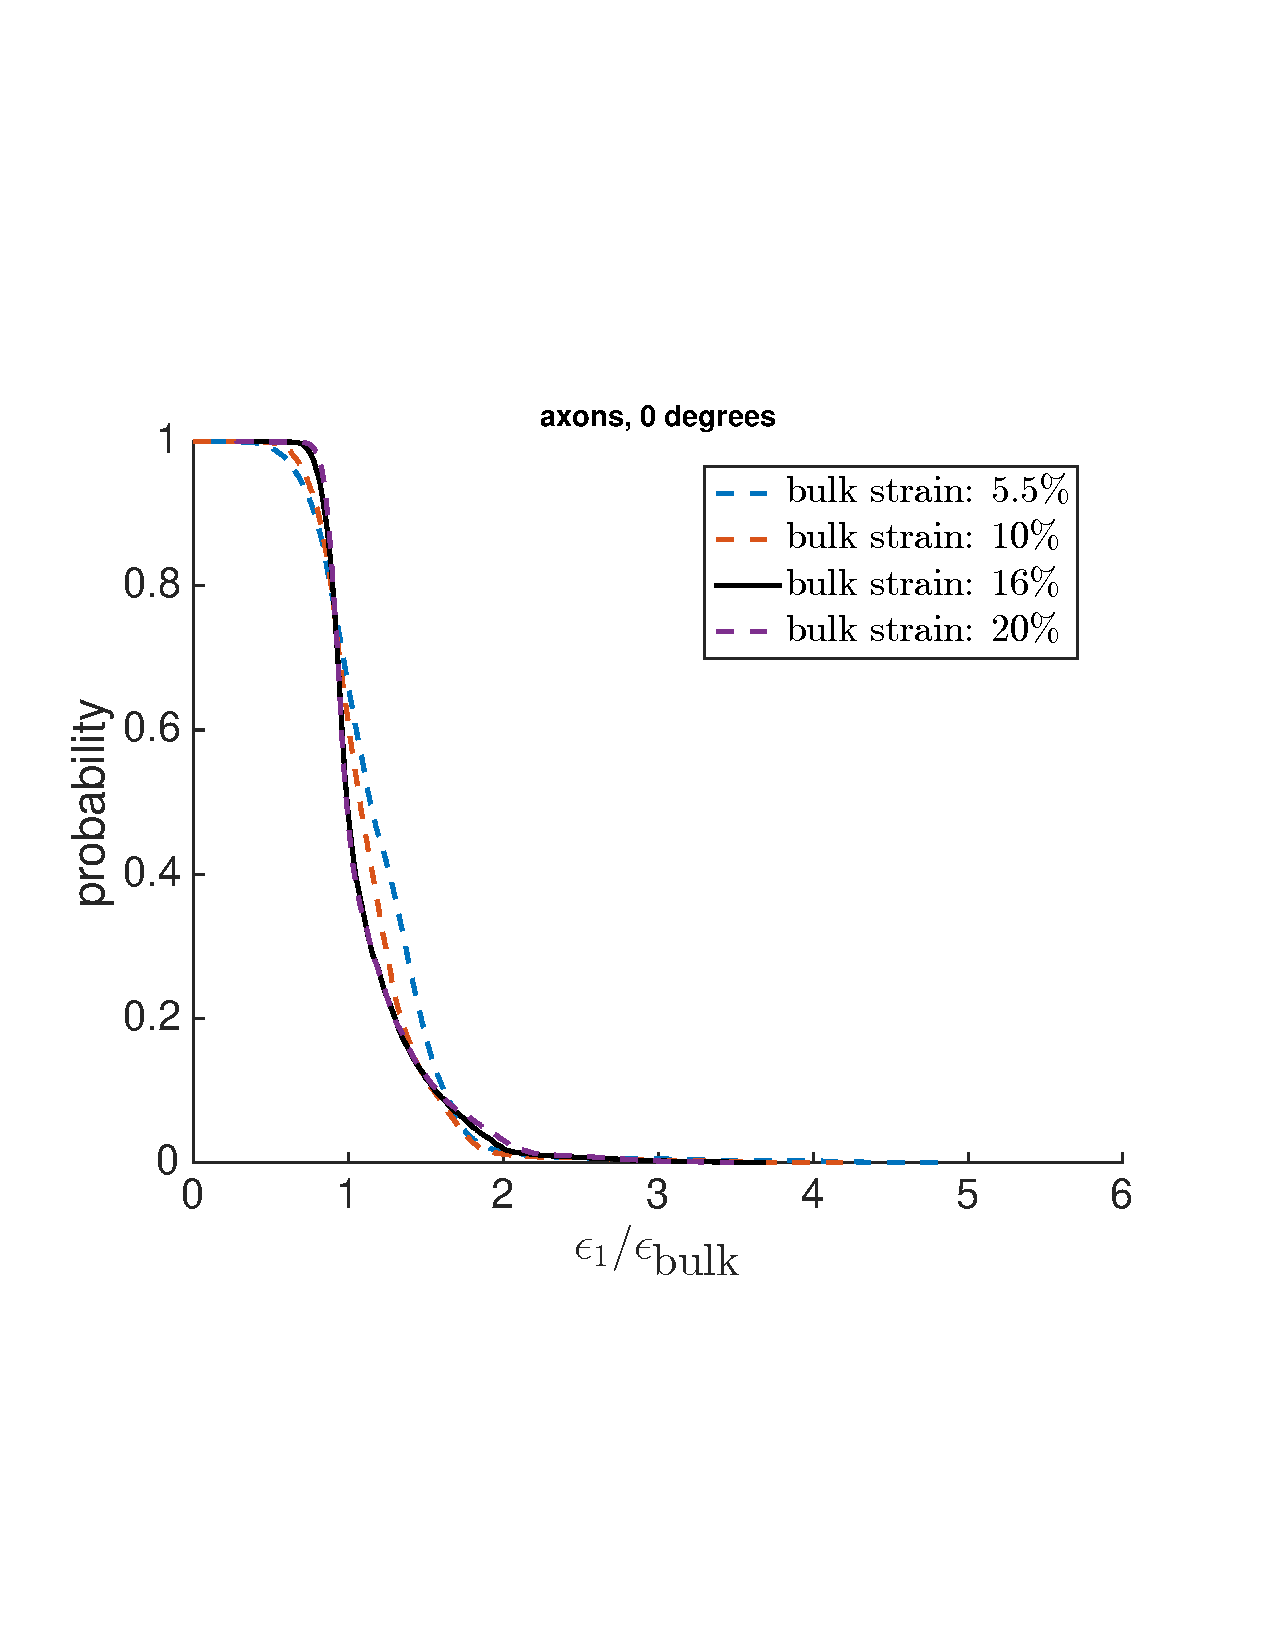
\includegraphics[height=4cm]{figure/rot0_FT50_128_1920_cdf_axons_compare_stps.pdf} &
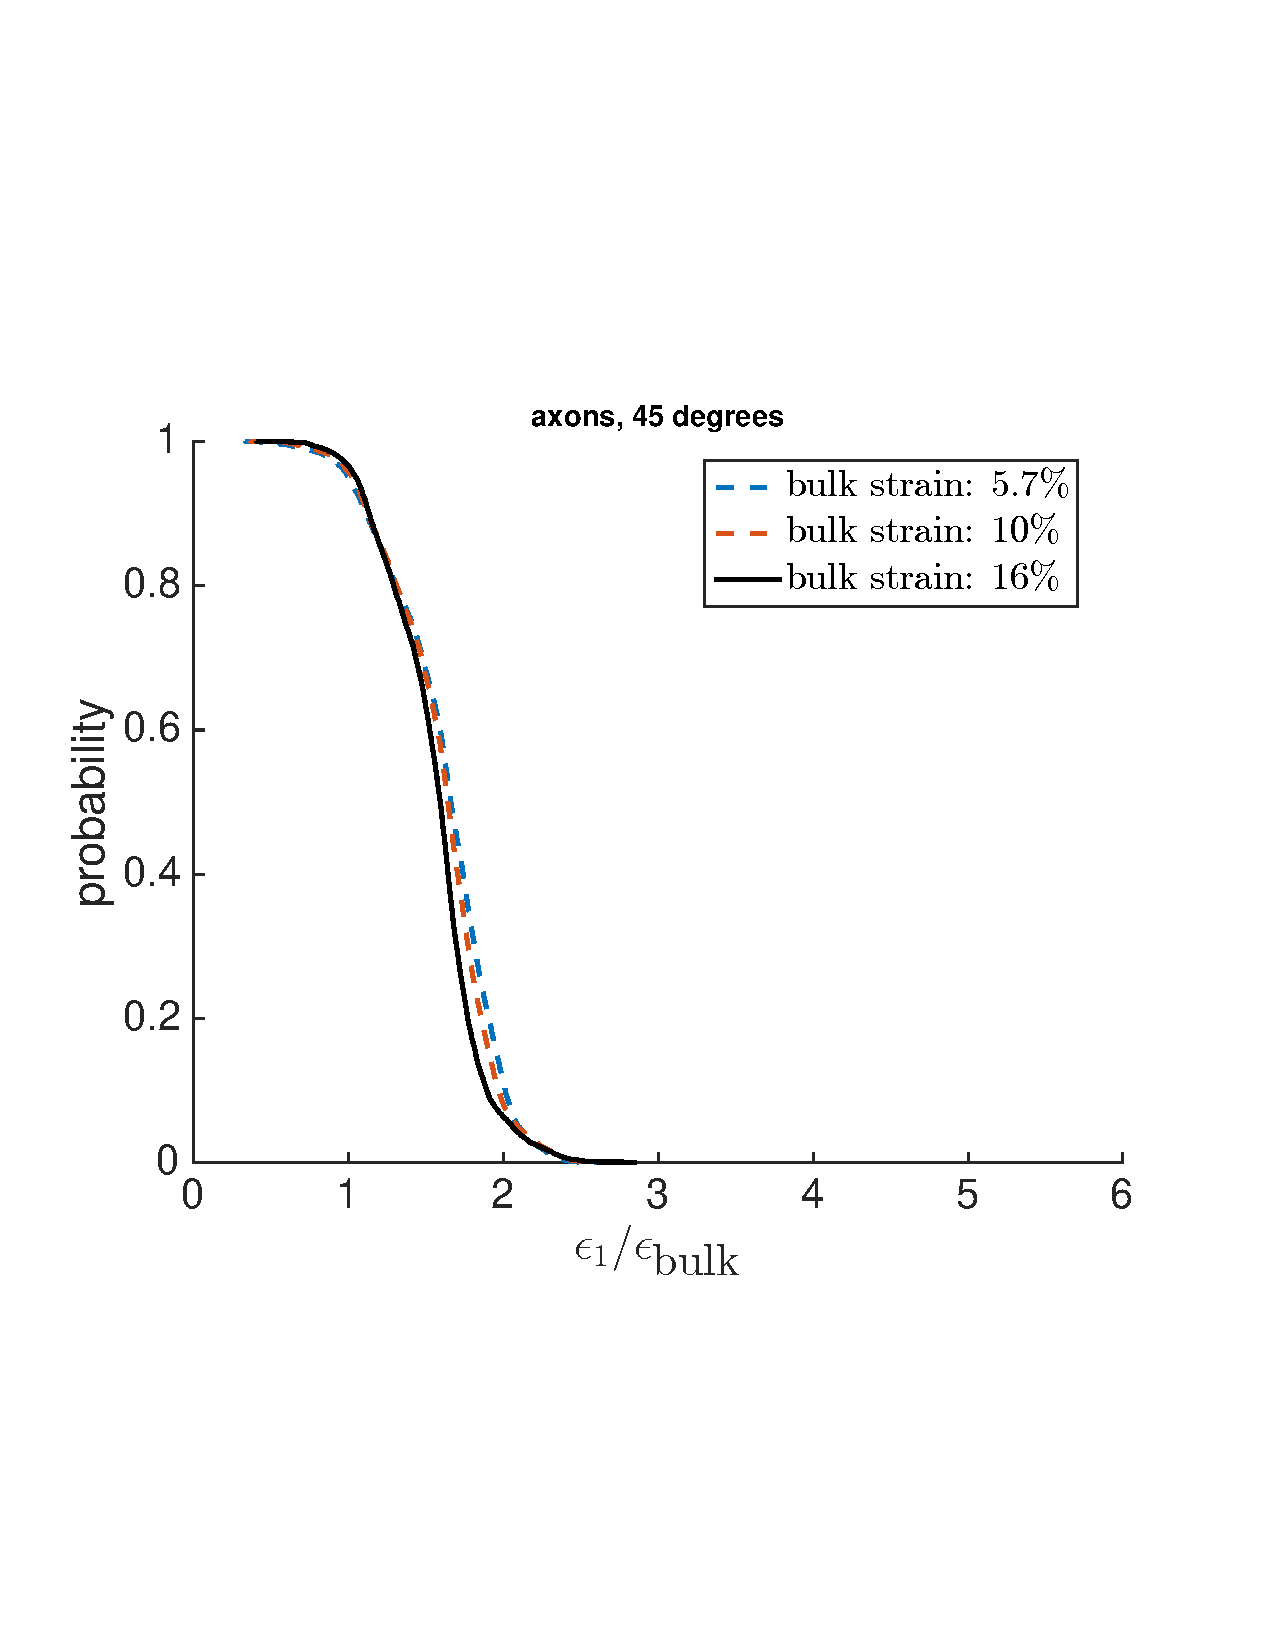
\includegraphics[height=4cm]{figure/rot45_FT50_128_1920_cdf_axons_compare_stps.pdf} &
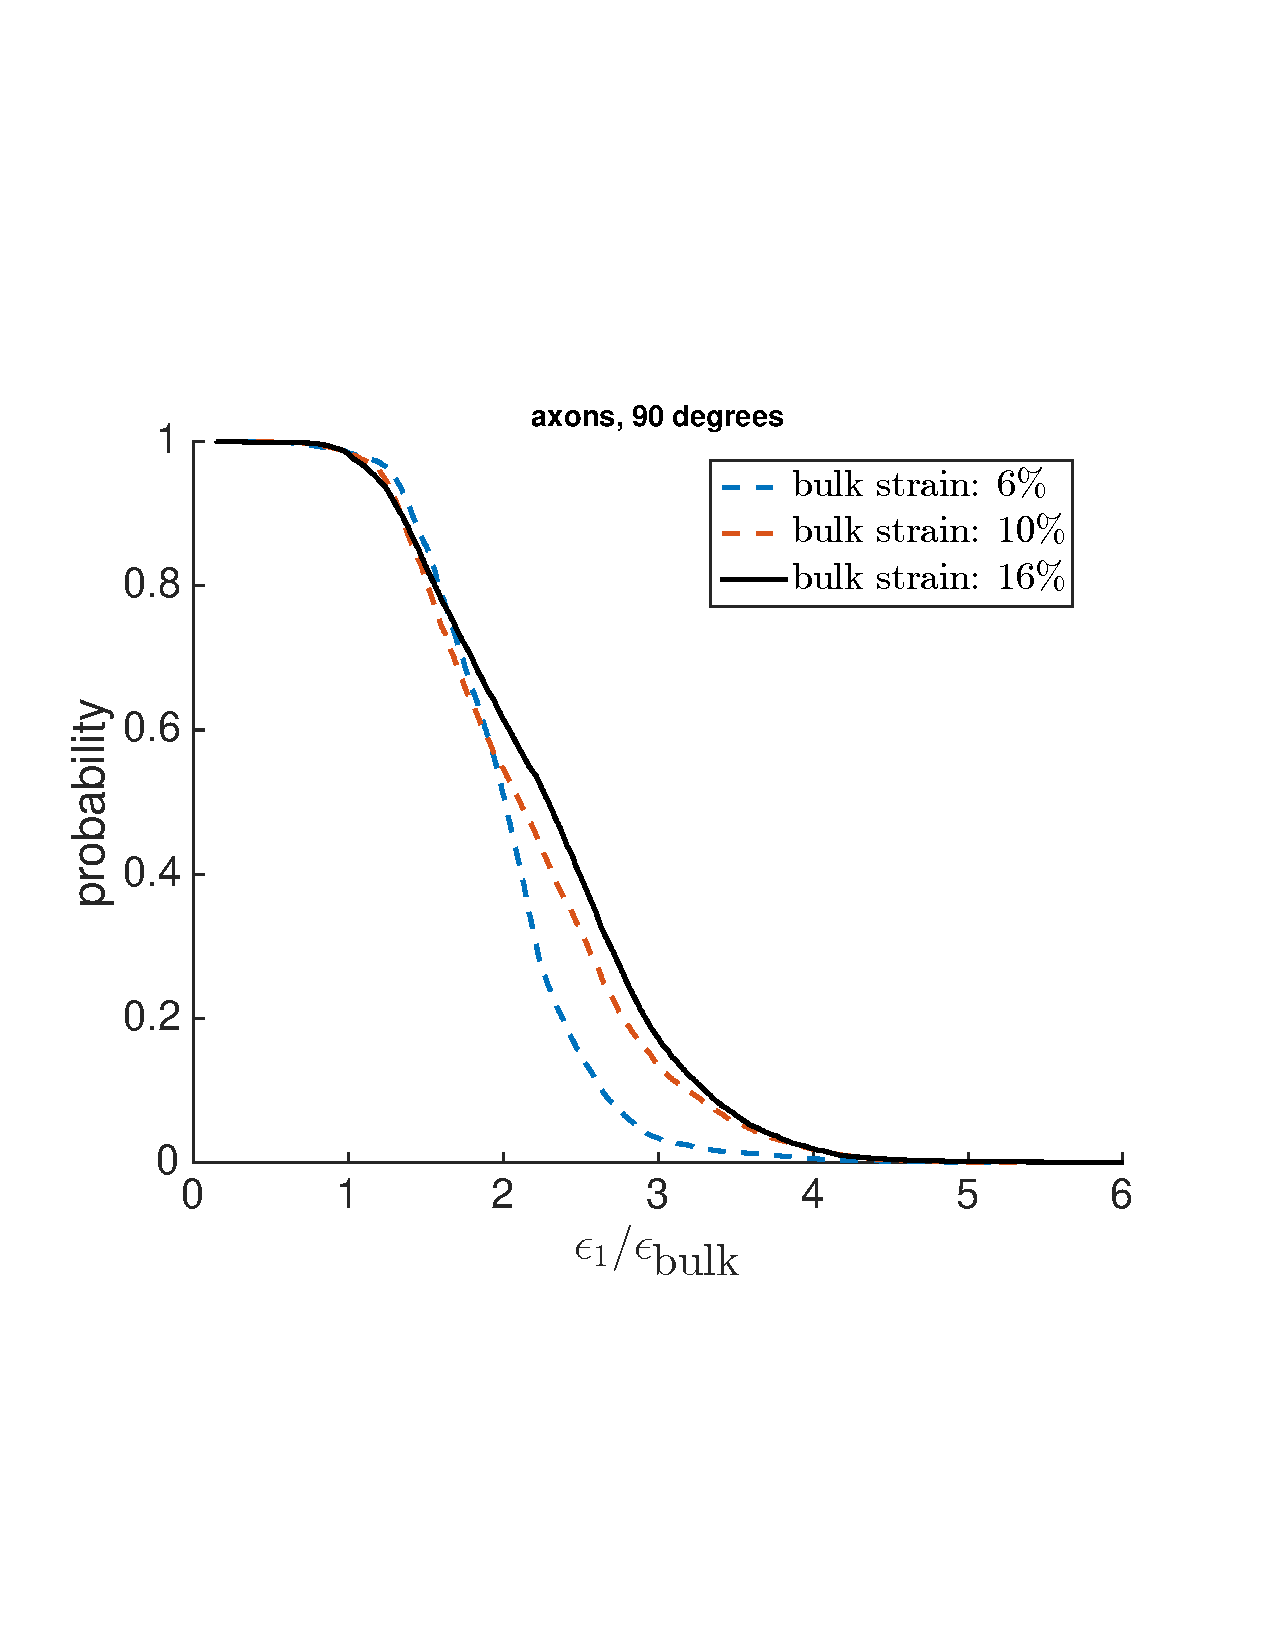
\includegraphics[height=4cm]{figure/rot90_FT_dspBC50_a30_128_1920_cdf_axons_compare_stps_farfield.pdf} \\
(d) & (e) & (f)
\end{array}
$
\end{center}
\caption{\label{fig:components_cdf} Complementary cdf of normalized maximum principal strain ($\varepsilon_1$) in the cell bodies for applied loads at (a) 0 degrees and (b) 90 degrees. For each angle, the complementary cdf for 6$\%$, 10$\%$, 16$\%$ (pain threshold), and 20$\%$ bulk strain is shown. The values of $\varepsilon_1$ are normalized by the applied bulk strain ($\varepsilon_{\text{bulk}}$) that is applied to the surrounding collagen gel. }
\end{figure}
%
The strain distribution in the cell bodies for the applied load at 45 degrees is essentially identical for all bulk strains, \textcolor{red}{which indicates the cell bodies are deforming affinely with the surrounding collagen gel.} For the same angle of applied load there is some slight variation in the distribution for the axon, which accounts for the small variations seen in the distribution of the neuron (see Fig.\ \ref{fig:neuron_cdf}(b)). For the applied load at 0 degrees, variations in the distributions of the cell bodies and axons for different bulk strains become more apparent. For the cell bodies, the distribution shifts to the right with larger bulk strains while the shape and spread of the distributions remain relatively constant. For the axons, the distributions shift to the left and the spread of the distributions decrease with larger bulk strains. The variations in the distributions of the cell bodies and axons ultimately cancel out leaving the overall distributions in the neuron relatively constant for different bulk strains (see Fig.\ \ref{fig:neuron_cdf}(a)). 

For the applied load at 90 degrees, the distributions of the cell bodies and axons shift to the right and the spread of the distributions grow with larger bulk strains. The subtle step feature of the distribution in the neuron (see Fig.\ \ref{fig:neuron_cdf}(c)) becomes apparent for the strain distributions in the cell bodies. This step feature indicates that there are two regimes of strain in the cell bodies, which are clearly seen in the plots of maximum principal strain in Figs.\ \ref{fig:neuron_MPS}(e) and (f) - the strain in the cell body that is parallel to the direction of applied load at 90 degrees is significantly lower than the other two cell bodies. 

\textcolor{red}{[The decrease in spread of the distribution with larger bulk strain indicates ...]}
%
\begin{figure}[ht]
\begin{center}
$
\begin{array}{cc}
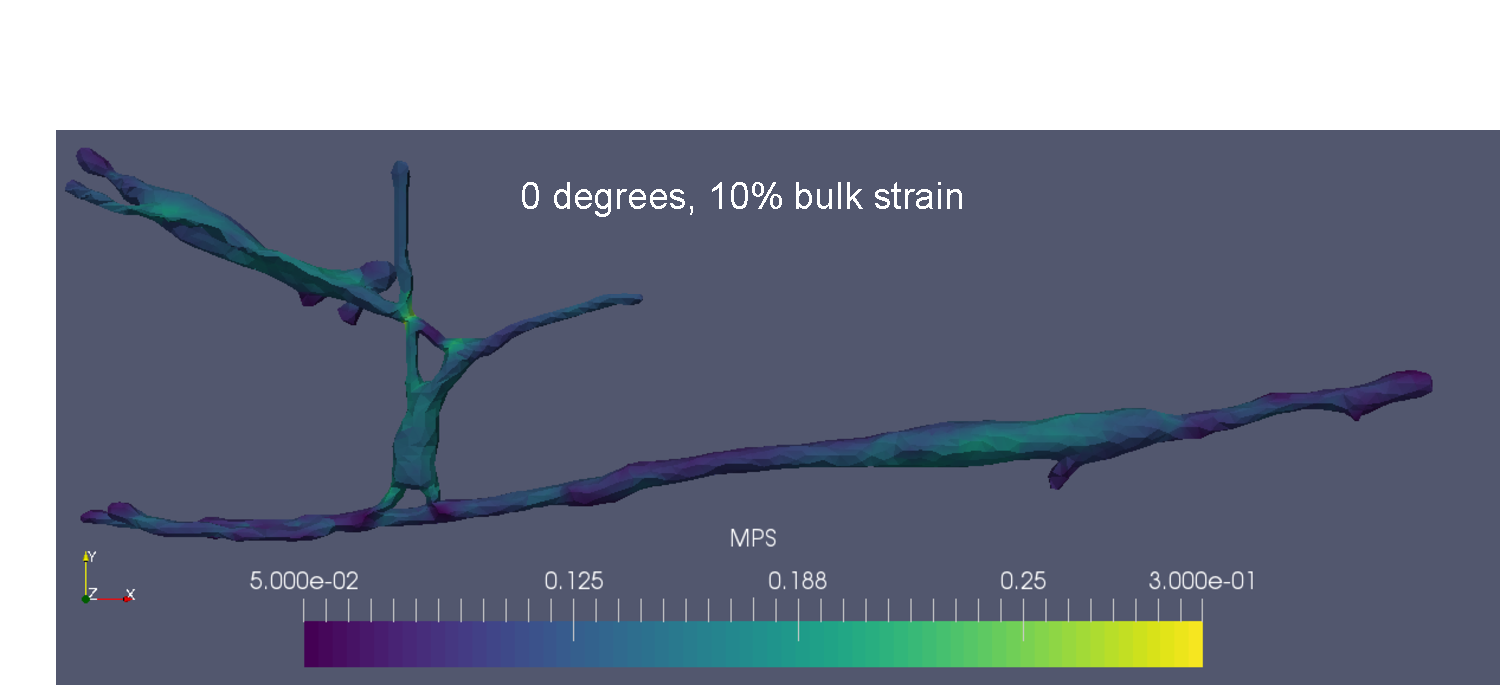
\includegraphics[width=8cm]{figure/MPS_rot0_strain10.pdf} & 
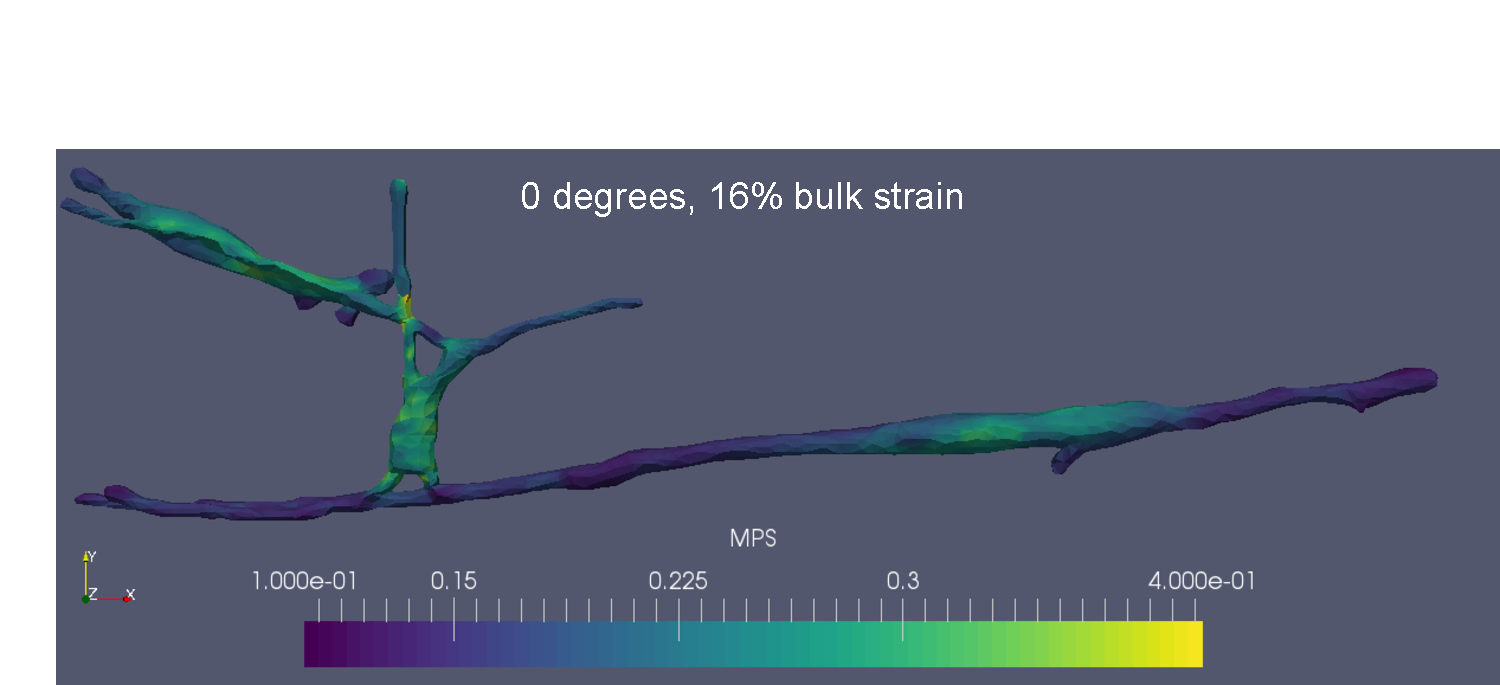
\includegraphics[width=8cm]{figure/MPS_rot0_strain16.pdf} \\
(a) & (b) \\ 
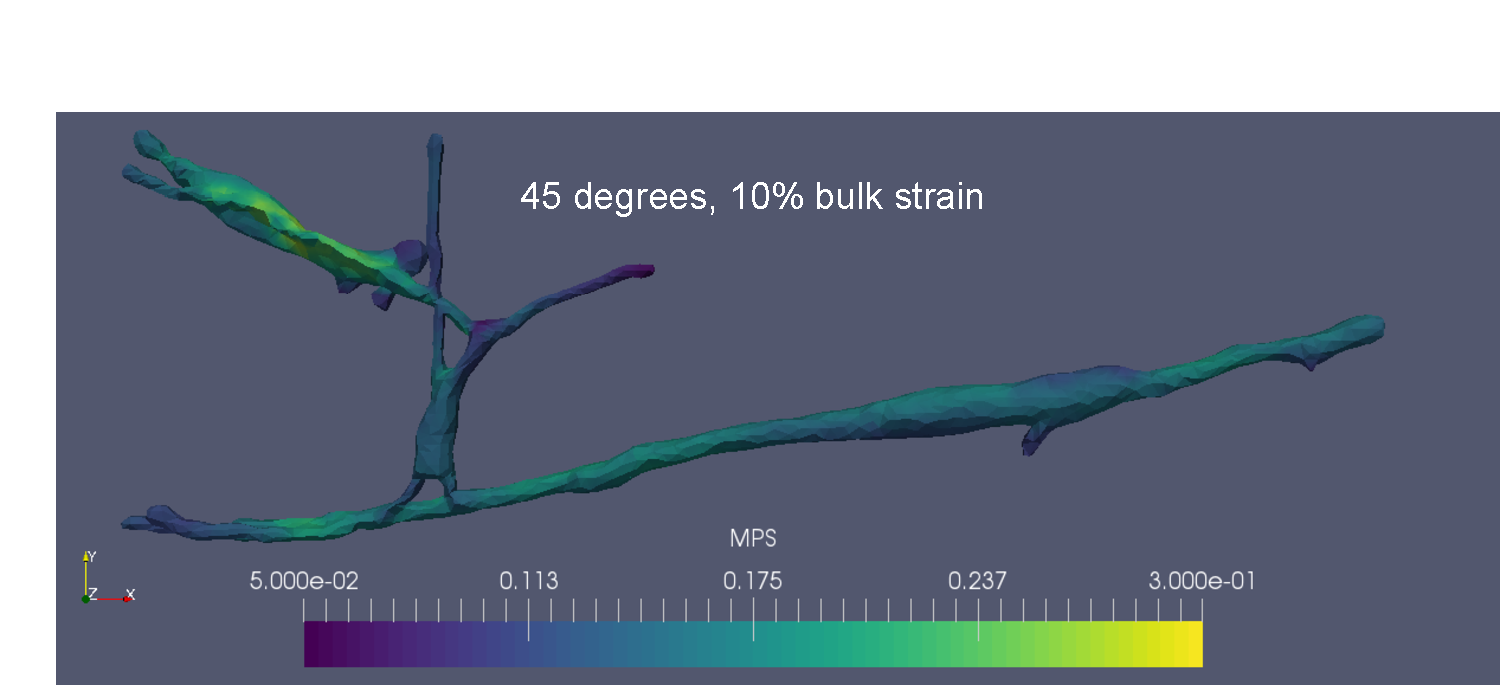
\includegraphics[width=8cm]{figure/MPS_rot45_strain10.pdf} &
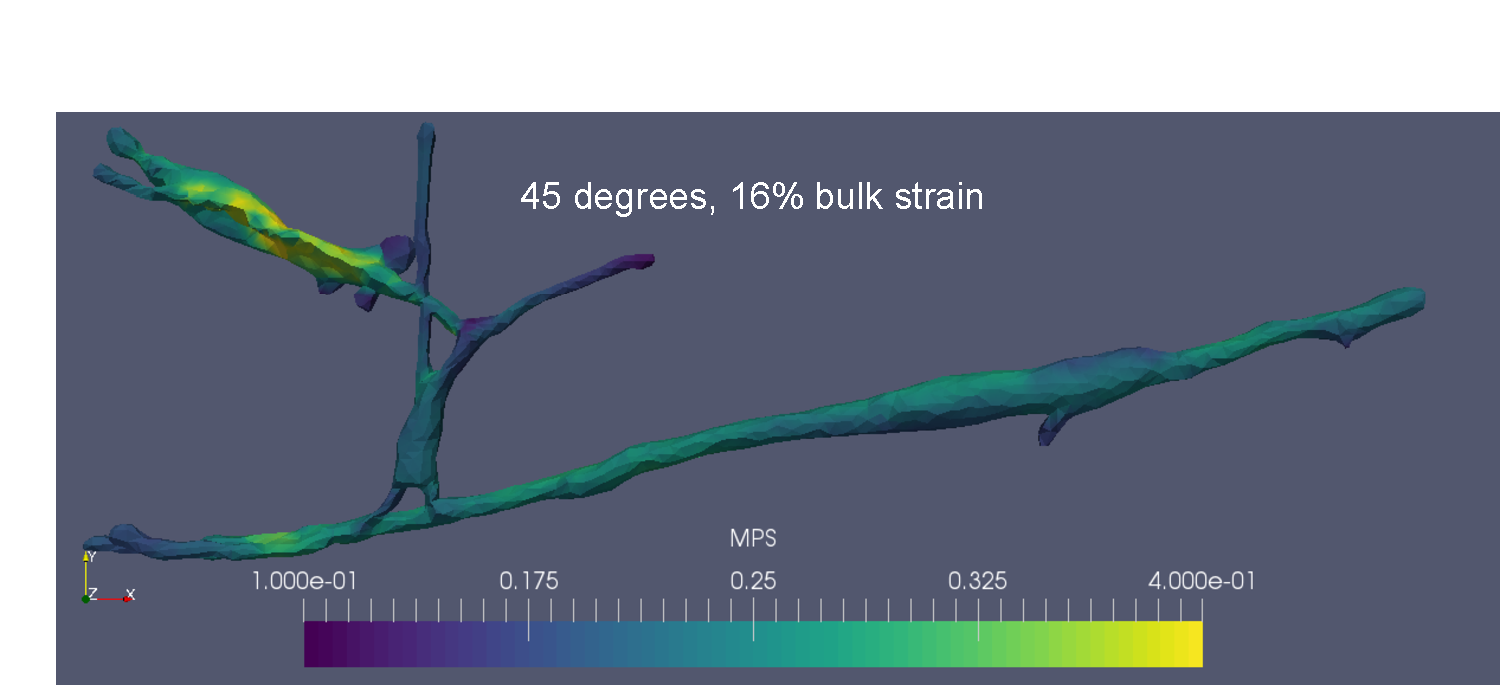
\includegraphics[width=8cm]{figure/MPS_rot45_strain16.pdf} \\
(c) & (d) \\
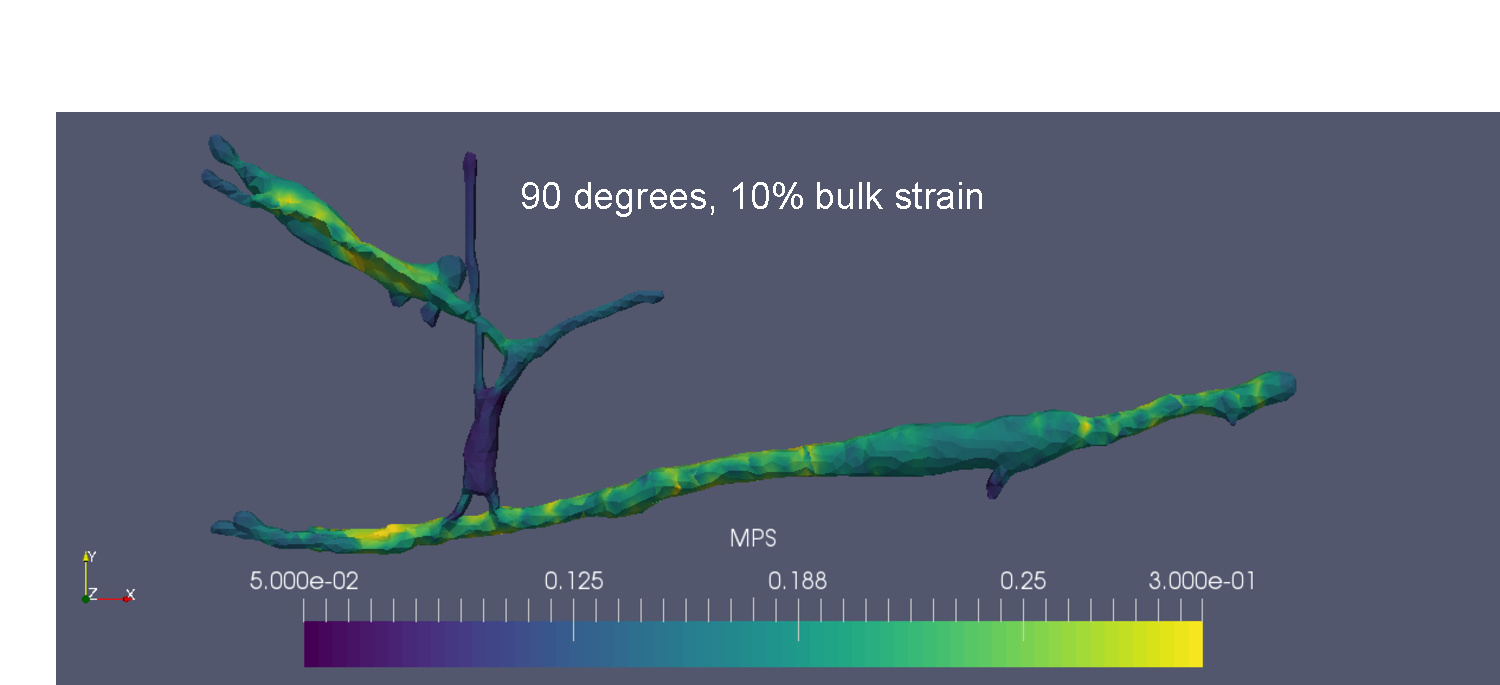
\includegraphics[width=8cm]{figure/MPS_rot90_strain10.pdf} & 
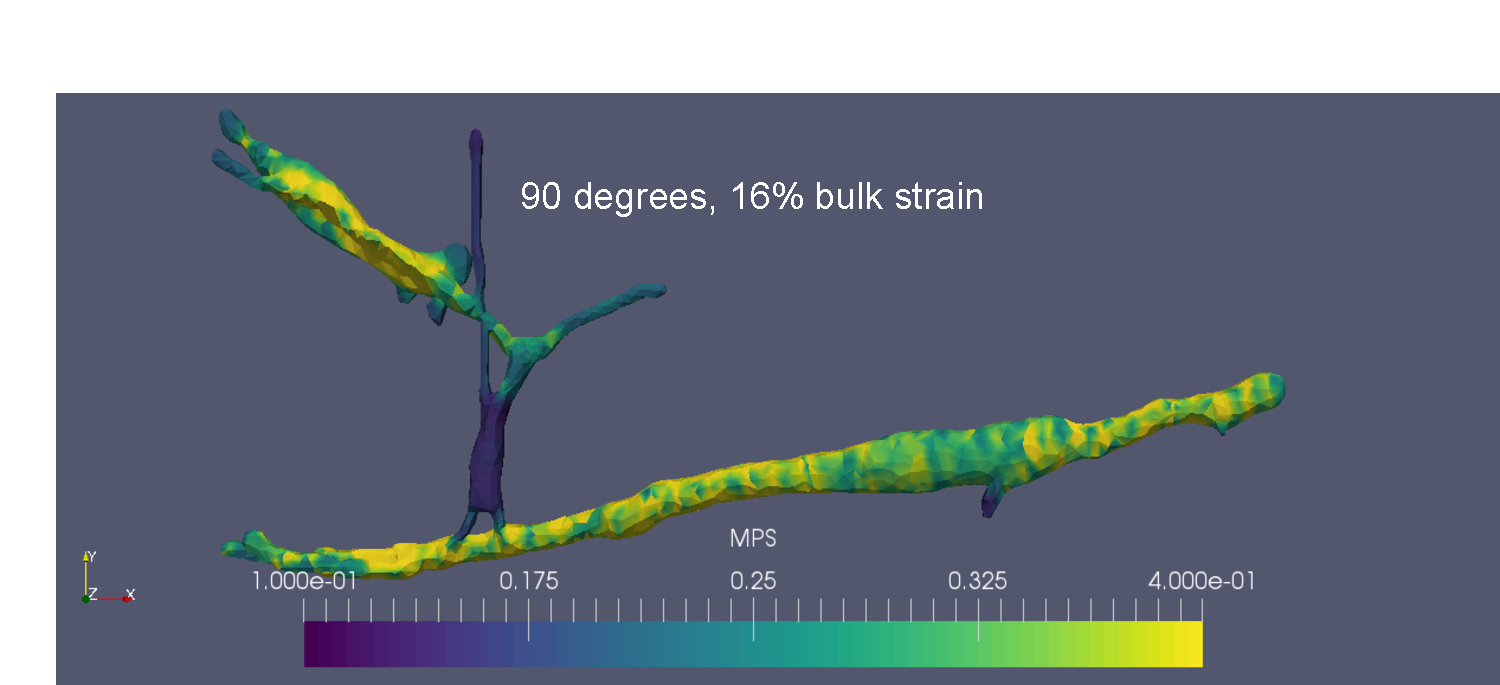
\includegraphics[width=8cm]{figure/MPS_rot90_strain16.pdf} \\
(e) & (f)
\end{array}
$
\end{center}
\caption{\label{fig:neuron_MPS} Complementary cdf of normalized maximum principal strain ($\varepsilon_1$) in the cell bodies for applied loads at (a) 0 degrees and (b) 90 degrees. For each angle, the complementary cdf for 6$\%$, 10$\%$, 16$\%$ (pain threshold), and 20$\%$ bulk strain is shown. The values of $\varepsilon_1$ are normalized by the applied bulk strain ($\varepsilon_{\text{bulk}}$) that is applied to the surrounding collagen gel. }
\end{figure}
%

In contrast to what is seen in the distribution for cell bodies, the spread in the distribution for the axons decreases for larger applied bulk strain at 0 degrees. Therefore, the decrease in the spread of the strain distribution in the neuron for larger applied bulk strain at 0 degrees is due primarily to the response of the axons. For the case where the applied load is at 90 degrees, 


\textcolor{red}{[Can explain the change in spread by looking at fiber alignment in the gel?]} In the case for the applied load at 90 degree,   

For both load angles, the overall shape of the distribution remains the same for the different values of bulk strain. For an applied load of 0 degrees, the distribution is relatively narrow with more than 90$\%$ of the neuron experience larger strain locally than the applied bulk strain on the collagen gel. For an applied load of 90 degrees, the distribution is significantly wider with two steps that indicate two regimes of strain in cell bodies. Additionally, for the applied load of 90 degrees, the strain distribution tightens as the applied bulk strain increases.


\subsection{Fiber Alignment in Collagen Gel}
The mechanical behavior observed in the neuron is influenced by the alignment of fibers in the collagen gel.
%
%\begin{figure}[ht]
%\begin{center}
%$
%\begin{array}{cc}
%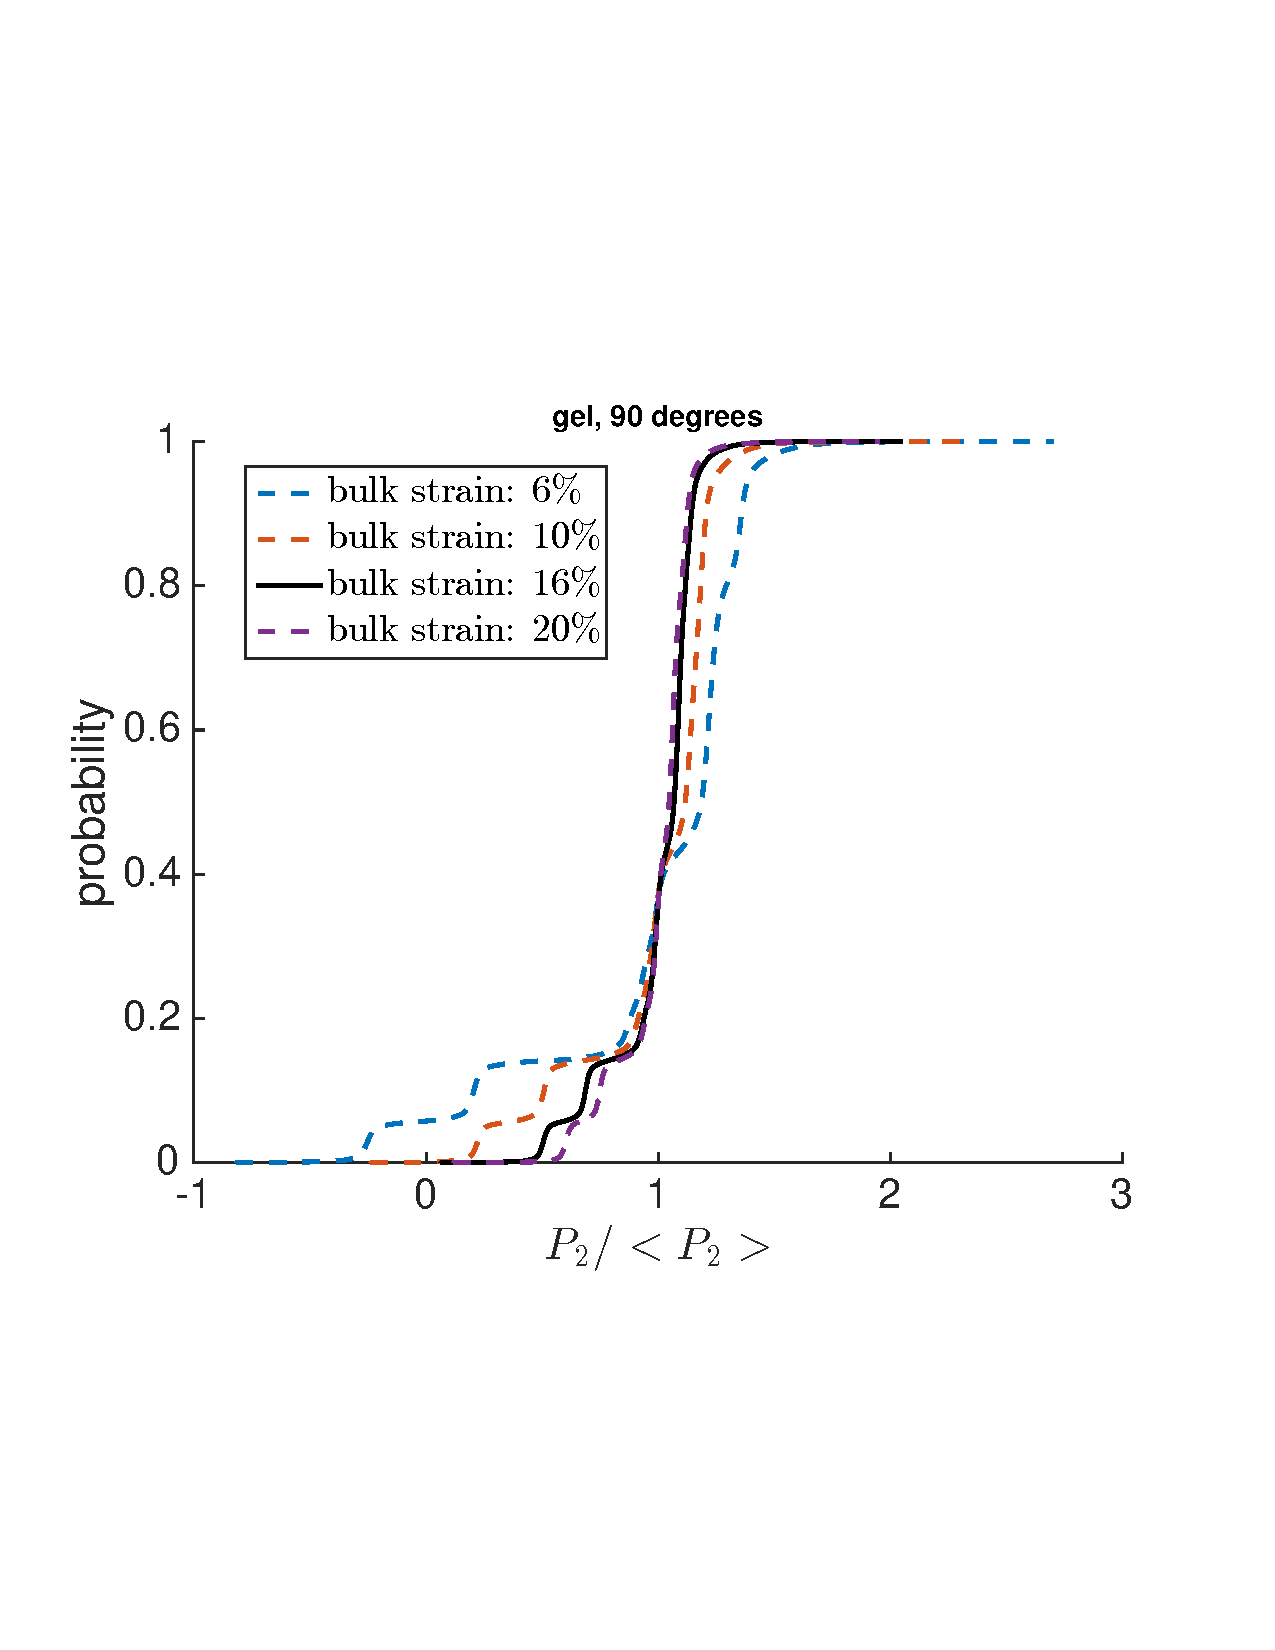
\includegraphics[height=5cm]{figure/rot0_FT_dspBC50_a30_128_1920_cdf_gel_compare_stps.pdf} &
%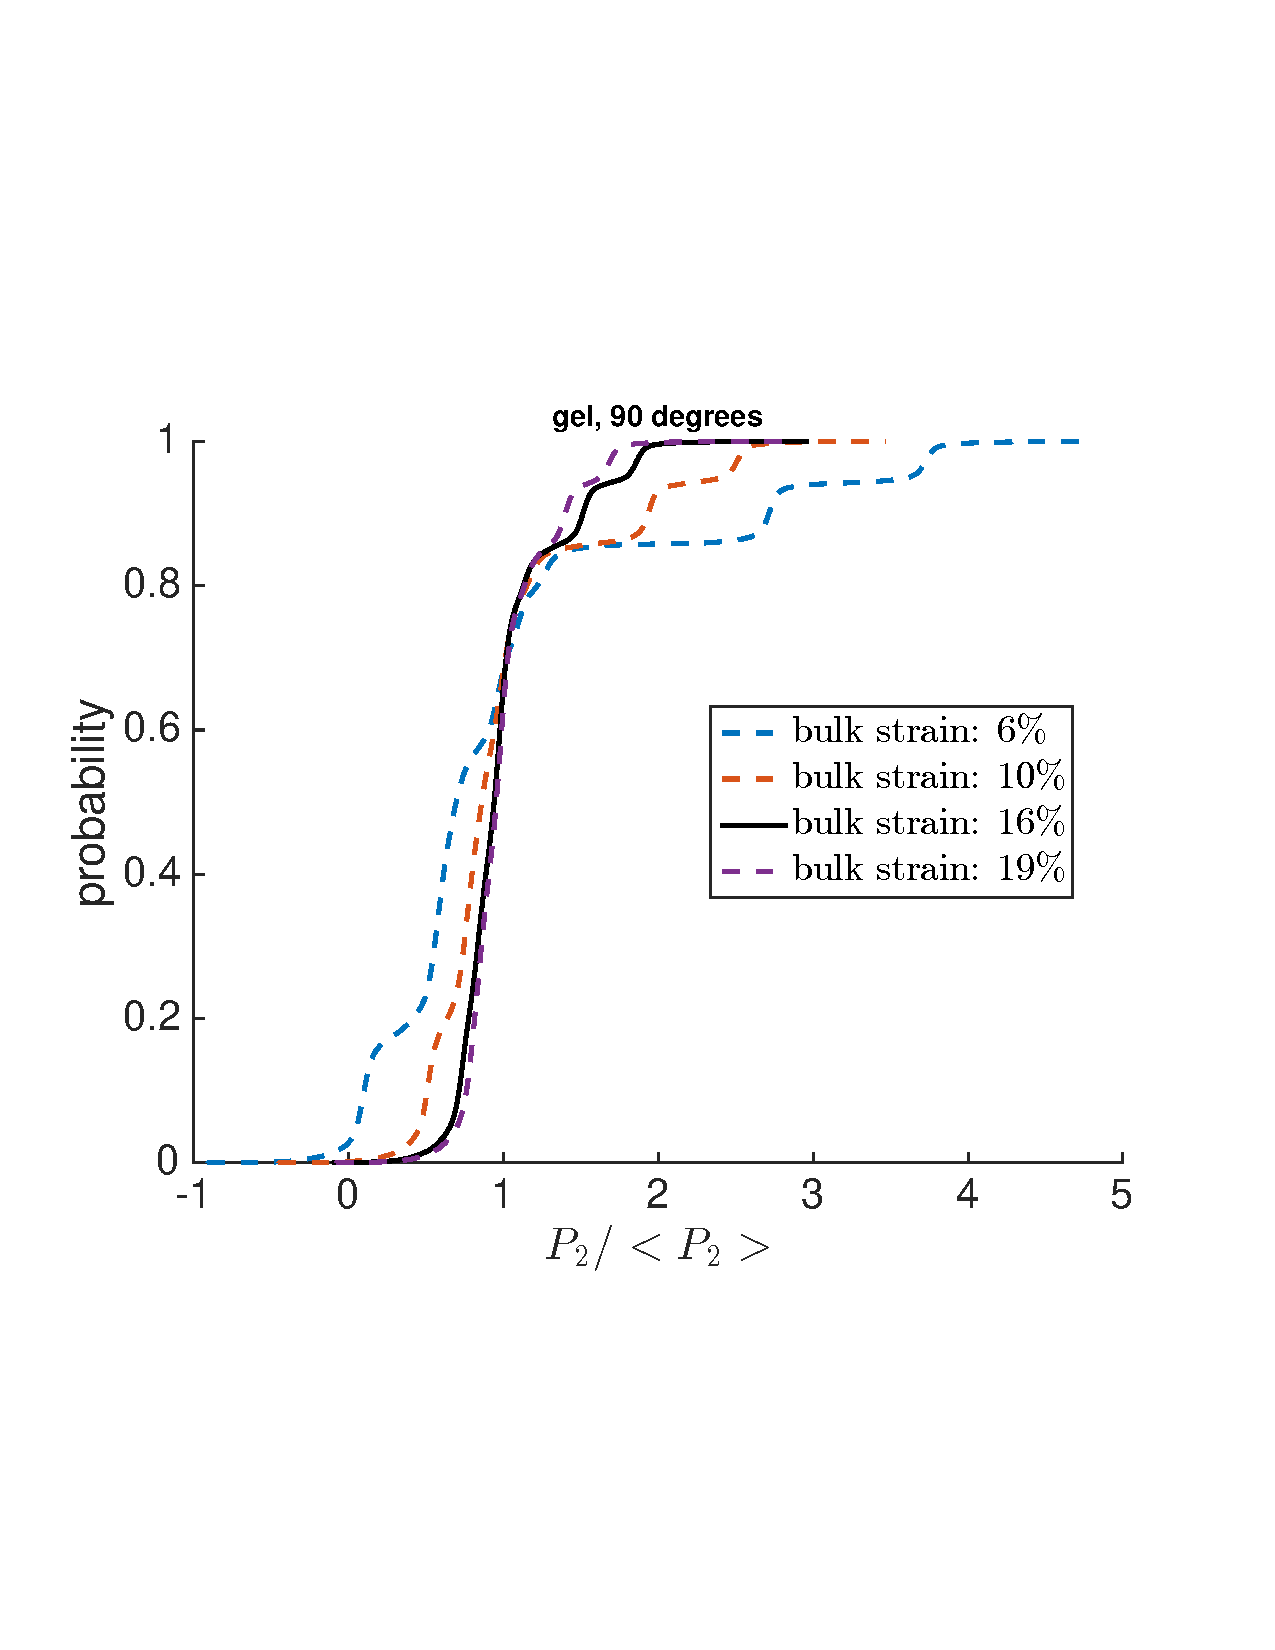
\includegraphics[height=5cm]{figure/rot90_FT_dspBC50_a30_128_1920_cdf_gel_compare_stps.pdf} \\
%(a) & (b)
%\end{array}
%$
%\end{center}
%\caption{\label{fig:gel_cdf} Plots of cdf normalized $P_2$ in collagen gel for applied loads at (a) 0 degrees and (b) 90 degrees. For each angle, the complementary cdf for 6, 10, 16 (pain threshold), and 20 percent bulk strain is shown. The values of $P_2$ are normalized its mean value. }
%\end{figure}
%
\subsection{Local Axial Coordinates, Cross-sectional Strain?}

%%%%%%%%%%%%%%%%%%%%%%%%%%%%%%%%%%%%%%%%%%%%%%%%%%%%%%%%%%%%%%%%%%%%%%
\section{Conclusion}

%%%%%%%%%%%%%%%%%%%%%%%%%%%%%%%%%%%%%%%%%%%%%%%%%%%%%%%%%%%%%%%%%%%%%%
\begin{acknowledgment}

\end{acknowledgment}

%%%%%%%%%%%%%%%%%%%%%%%%%%%%%%%%%%%%%%%%%%%%%%%%%%%%%%%%%%%%%%%%%%%%%%
% The bibliography is stored in an external database file
% in the BibTeX format (file_name.bib).  The bibliography is
% created by the following command and it will appear in this
% position in the document. You may, of course, create your
% own bibliography by using thebibliography environment as in
%
% \begin{thebibliography}{12}
% ...
% \bibitem{itemreference} D. E. Knudsen.
% {\em 1966 World Bnus Almanac.}
% {Permafrost Press, Novosibirsk.}
% ...
% \end{thebibliography}
\newpage
% Here's where you specify the bibliography style file.
% The full file name for the bibliography style file 
% used for an ASME paper is asmems4.bst.
\bibliographystyle{asmems4}

% Here's where you specify the bibliography database file.
% The full file name of the bibliography database for this
% article is asme2e.bib. The name for your database is up
% to you.
\bibliography{references}


\end{document}
